\documentclass[12pt,a4paper,oneside]{book}
\usepackage[utf8x]{vietnam}
\usepackage{amsmath, amsthm, amssymb,latexsym,amscd,amsfonts,enumerate,titlesec,titletoc}
\usepackage[top=3.5cm, bottom=3.0cm, left=3.5cm, right=2.0cm]{geometry}
% căn lề theo quy chuẩn KLTN
\usepackage{color, fancyhdr, graphicx, wrapfig}
\usepackage[colorlinks=true,linkcolor=black,anchorcolor=black,citecolor=black,filecolor=black,menucolor=black,runcolor=black,urlcolor=black,unicode]{hyperref}
%\usepackage[unicode]{hyperref}
\usepackage{indentfirst}
\usepackage{graphicx}
\usepackage{float}
\usepackage{multirow}
\usepackage[thinlines]{easytable}
\usepackage{array}
\usepackage{etoolbox}% http://ctan.org/pkg/etoolbox
\usepackage{subfig} 
\usepackage{tocbasic}
\captionsetup{labelfont=bf}
\usepackage{url}
\usepackage{etoolbox}
\usepackage{booktabs}% http://ctan.org/pkg/booktabs
\usepackage{textcomp}
\usepackage{capt-of} 

\newcommand{\tabitem}{~~\llap{\textbullet}~~}

%\usepackage[labelfont=bf]{caption}

\def\chaptertitlename{\fontsize{14pt}{14pt}\selectfont{CHƯƠNG}}
\titleformat{\chapter}[display]
{\vspace{-2cm}\normalfont\Large\filcenter\bfseries}
{{{\chaptertitlename\,}\thechapter}} {0pc}{{}\MakeUppercase}

\newcolumntype{P}[1]{>{\centering\arraybackslash}p{#1}}


\pagestyle{fancy}
\makeatletter
\renewcommand{\ps@plain}{
\renewcommand{\@oddfoot}{\textrm{\centerline{\thepage}}}
\renewcommand{\@evenhead}{\@oddhead}
%\renewcommand{\@oddfoot}{}
\renewcommand{\@evenfoot}{\@oddfoot}}

\pagestyle{plain}

%%%%%%%%%%%%%%%%%
\begin{document}


\fontsize{14pt}{25pt}\selectfont % Lệnh thay đổi cỡ chữ thành cỡ 14, cỡ dòng 18 (theo quy chuẩn của Khóa Luận TN).
\setlength{\baselineskip}{26truept}
%\fontsize{13pt}{14pt}\selectfont
\pagenumbering{arabic}
%\pagenumbering{roman}
%\frontmatter
\pagestyle{empty}
\begin{titlepage}
	\centerline{ĐẠI HỌC QUỐC GIA THÀNH PHỐ HỒ CHÍ MINH}
	\centerline{\bf\underline{TRƯỜNG ĐẠI HỌC CÔNG NGHỆ THÔNG TIN}}
	\centerline{\bf KHOA KHOA HỌC \& KỸ THUẬT THÔNG TIN}
	\vspace{3.0cm}
	\centerline{\bf\fontsize{20pt}{16}\selectfont BÁO CÁO ĐỒ ÁN CUỐI KỲ}
	\centerline{\bf\fontsize{14.5pt}{16}\selectfont MÔN: HỌC MÁY THỐNG KÊ}
	\centerline{\bf\fontsize{14.5pt}{16}\selectfont LỚP: DS102.L21}
	\vspace{2.5cm}
	\begin{center}{\bf\fontsize{20pt}{28}\selectfont BÀI TOÁN NHẬN DIỆN TIN GIẢ \\FAKE NEWS DETECTION PROJECT}
	\end{center}
	\vspace{2cm}
	\center{ Sinh viên thực hiện}\\ \center{\textbf{Thái Minh Triết - 19522397\\Chu Hà Thảo Ngân - 19521882}}
	\vfill
	\centerline{\bf Thành phố Hồ Chí Minh - 07/2020}
\end{titlepage}
\newpage

\begin{titlepage}
	\centerline{ĐẠI HỌC QUỐC GIA THÀNH PHỐ HỒ CHÍ MINH}
	\centerline{\bf\underline{TRƯỜNG ĐẠI HỌC CÔNG NGHỆ THÔNG TIN}}
	\centerline{\bf KHOA KHOA HỌC \& KỸ THUẬT THÔNG TIN}
	\vspace*{3.0cm}
	\centerline{\bf\fontsize{20pt}{16}\selectfont BÁO CÁO ĐỒ ÁN CUỐI KỲ}
	\centerline{\bf\fontsize{14.5pt}{16}\selectfont MÔN: HỌC MÁY THỐNG KÊ}
	\centerline{\bf\fontsize{14.5pt}{16}\selectfont LỚP: DS102.L21}
	\vspace*{2.5cm}
	\begin{center}{\bf\fontsize{20pt}{28}\selectfont BÀI TOÁN NHẬN DIỆN TIN GIẢ\\ FAKE NEWS DETECTION PROJECT}\\
	\end{center}
	\vspace{2cm}
	\center{ Giảng viên hướng dẫn}\\ \center{\textbf{TS. Nguyễn Tấn Trần Minh Khang\\ThS. Võ Duy Nguyên}}
	\vfill
	\centerline{\bf Thành phố Hồ Chí Minh - 07/2020}
\end{titlepage}

\newpage

\newpage
\def\@chapter[#1]#2{\ifnum \c@secnumdepth >\m@ne
                       \if@mainmatter
                         \refstepcounter{chapter}%
                         \typeout{\@chapapp\space\thechapter.}%
                         \addcontentsline{toc}{chapter}%
                              {\bf  Chương \protect\numberline{\thechapter. } #1}%
                       \else
                         \addcontentsline{toc}{chapter}{ #1}%
                       \fi
                    \else
                      \addcontentsline{toc}{chapter}{ #1}%
                    \fi
                    \chaptermark{#1}%
                    \addtocontents{lof}{\protect\addvspace{10\p@}}%
                    \addtocontents{lot}{\protect\addvspace{10\p@}}%
                    \if@twocolumn
                      \@topnewpage[\@makechapterhead{#2}]%
                    \else
                      \@makechapterhead{#2}%
                      \@afterheading
                    \fi}
%\setcounter{page}{3}
%%%%%%%%%%%%%%%%%%%%%%%
%\pagenumbering{roman}
\markboth{{\it Mục lục}}{{\it Mục lục}}
%\addcontentsline{toc}{section}{{\bf Mục lục\rm }}
%\cleardoublepage
\tableofcontents
\addtocontents{toc}{\protect\thispagestyle{empty}}
%{\protect\thispagestyle{empty}}

\makeatletter
\patchcmd{\@chapter}{\addtocontents{lof}{\protect\addvspace{10\p@}}}{}{}{}% LoF
\patchcmd{\@chapter}{\addtocontents{lot}{\protect\addvspace{10\p@}}}{}{}{}% LoT
\makeatother

\renewcommand*{\listfigurename}{DANH MỤC HÌNH ẢNH}
\listoffigures
\thispagestyle{empty}

\renewcommand*{\listtablename}{DANH MỤC BẢNG BIỂU}
\listoftables
\thispagestyle{empty}
%%%%%%%%%%%%%%

\pagestyle{plain}
\chapter*{LỜI CẢM ƠN}
	\addcontentsline{toc}{chapter}{LỜI CẢM ƠN}
	Lời đầu tiên, chúng tôi xin trân trọng cảm ơn hai Thầy giảng viên hướng dẫn là TS. Nguyễn Tấn Trần Minh Khang và ThS. Võ Duy Nguyên, các Thầy đã tận tình giảng dạy chúng tôi trong suốt quá trình học tập môn Học máy thống kê cũng như đã hướng dẫn chúng tôi hoàn thành đồ án của môn học này.
	
	Xin cảm ơn anh Hồ Thái Ngọc (PMCL2016) đã có sự giúp đỡ tận tình trong các tiết học lý thuyết và thực nghiệm tại lớp.
	
	Do giới hạn về kiến thức và khả năng lý luận còn nhiều hạn chế, kính mong sự chỉ dẫn và đóng góp của các quý Thầy để bài báo cáo của chúng tôi được hoàn thiện hơn. Xin chân thành cảm ơn!
	\vskip 1,5cm
	\hskip 9cm {\bf Nhóm sinh viên
	\vskip 1,5cm
	\hskip 9cm Thái Minh Triết
	
	\hskip 8.6cm Chu Hà Thảo Ngân
	}

\chapter*{NHẬN XÉT CỦA GIẢNG VIÊN HƯỚNG DẪN}
	\addcontentsline{toc}{chapter}{NHẬN XÉT CỦA GIẢNG VIÊN HƯỚNG DẪN}
	
\chapter*{TÓM TẮT}
	\addcontentsline{toc}{chapter}{TÓM TẮT}
%%%%%%%%%%%%%%%%%%%%%%%%

	Trong kỷ nguyên của Internet và mạng xã hội, cứ mỗi giây trôi qua, thế giới có gần 55.000 bài đăng trên Facebook, 456.000 tweet được gửi đi trên Twitter và có 86 bài blog xuất hiện trên Internet. Có thể thấy lượng thông tin được sản sinh ra và lan truyền nhanh chóng như thế nào trên không gian mạng. Tuy nhiên, những nguồn tin này luôn tiềm ẩn những thông tin giả mạo mà nếu không nhận diện và ngăn chặn kịp thời sẽ gây tổn hại đến đến các cá nhân, tổ chức chính trị, kinh tế và xã hội. 


	Các phương pháp nhận diện tin giả trước đây thường mang tính thủ công khi phải cần đến các chuyên gia để có thể thẩm định nguồn tin. Bên cạnh đó, các phương pháp nhận diện tự động ứng dụng lý thuyết Học máy và Xử lý ngôn ngữ tự nhiên là những hướng tiếp cận mới, trở thành xu hướng nghiên cứu nóng hổi vì mang lại hiệu quả cao, tiết kiệm thời gian và chi phí, vốn là những mặt còn nhiều hạn chế của các phương pháp cũ.


	Trong đồ án này, chúng tôi tiến hành thực nghiệm những phương pháp Học máy thường dùng cho bài toán phân loại, cùng các mô hình trích xuất đặc trưng từ dữ liệu văn bản, bao gồm 2 mô hình Bag-of-Words là TFIDFVectorizer và CountVectorizer cùng mô hình Word2Vec, với mục tiêu tìm hiểu khả năng trích xuất thông tin từ bộ dữ liệu cũng như độ hiệu quả của từng phương pháp trong việc phân loại một mẩu tin là đáng tin cậy hay là sai sự thật.

	\vspace{0.5cm}
	\textbf{Từ khóa: Machine Learning, Fake News Detection, Natural Language Processing, Classification, Word Embedding}
	\pagebreak
	
\chapter{GIỚI THIỆU CHUNG}

	\section{Mục tiêu đề tài}
	Mục tiêu đặt ra của đồ án này nhằm tìm hiểu và xây dựng các mô hình Học máy để nhận diện tin tức giả bằng cách phân loại các tin tức từ bộ dữ liệu theo 2 nhãn: REAL (tin thật) và FAKE (tin giả). Những mô hình Học máy mà chúng tôi khảo sát trong đồ án này dựa trên 6 phương pháp sau đây: Logistic Regression, Multinomial Naive Bayes, Support Vector Machine, Passive Aggressive, Decision Tree và Random Forest.
	
	Ngoài ra, mục tiêu của đề tài còn nhằm tìm hiểu và so sánh khả năng trích xuất thông tin của một số bộ trích chọn đặc trưng gồm TFIDFVectorizer, Countvectorizer và Word2Vec, cũng như độ hiệu quả của chúng trên các mô hình Học máy khác nhau. Qua đó có thể tìm ra mô hình và bộ vector hóa mang lại hiệu suất cao nhất trên bộ dữ liệu.
	
	\section{Bài toán học máy}
	Bài toán Nhận diện tin giả là một dạng điển hình của bài toán Supervised Learning (Học có giám sát), vì bộ dữ liệu sử dụng cho bài toán cần được gán nhãn rõ ràng. 
	
	Với việc phân loại tin thật và tin giả thì có thể thấy đây là một bài toán Phân lớp nhị phân (Binary Classification) với đầu vào và đầu ra như sau:
	\begin{itemize}
	\item \textbf{Input:} Thông tin về tiêu đề và nội dung của một tin tức.
	\item \textbf{Output:} Một trong hai nhãn: FAKE (hay 0) nếu dự đoán là tin giả, REAL (hay 1) nếu dự đoán là tin thật.
	\end{itemize}
	
	\section{Quy trình thực hiện bài toán}
	
	\begin{figure}[H]
		\begin{center}
			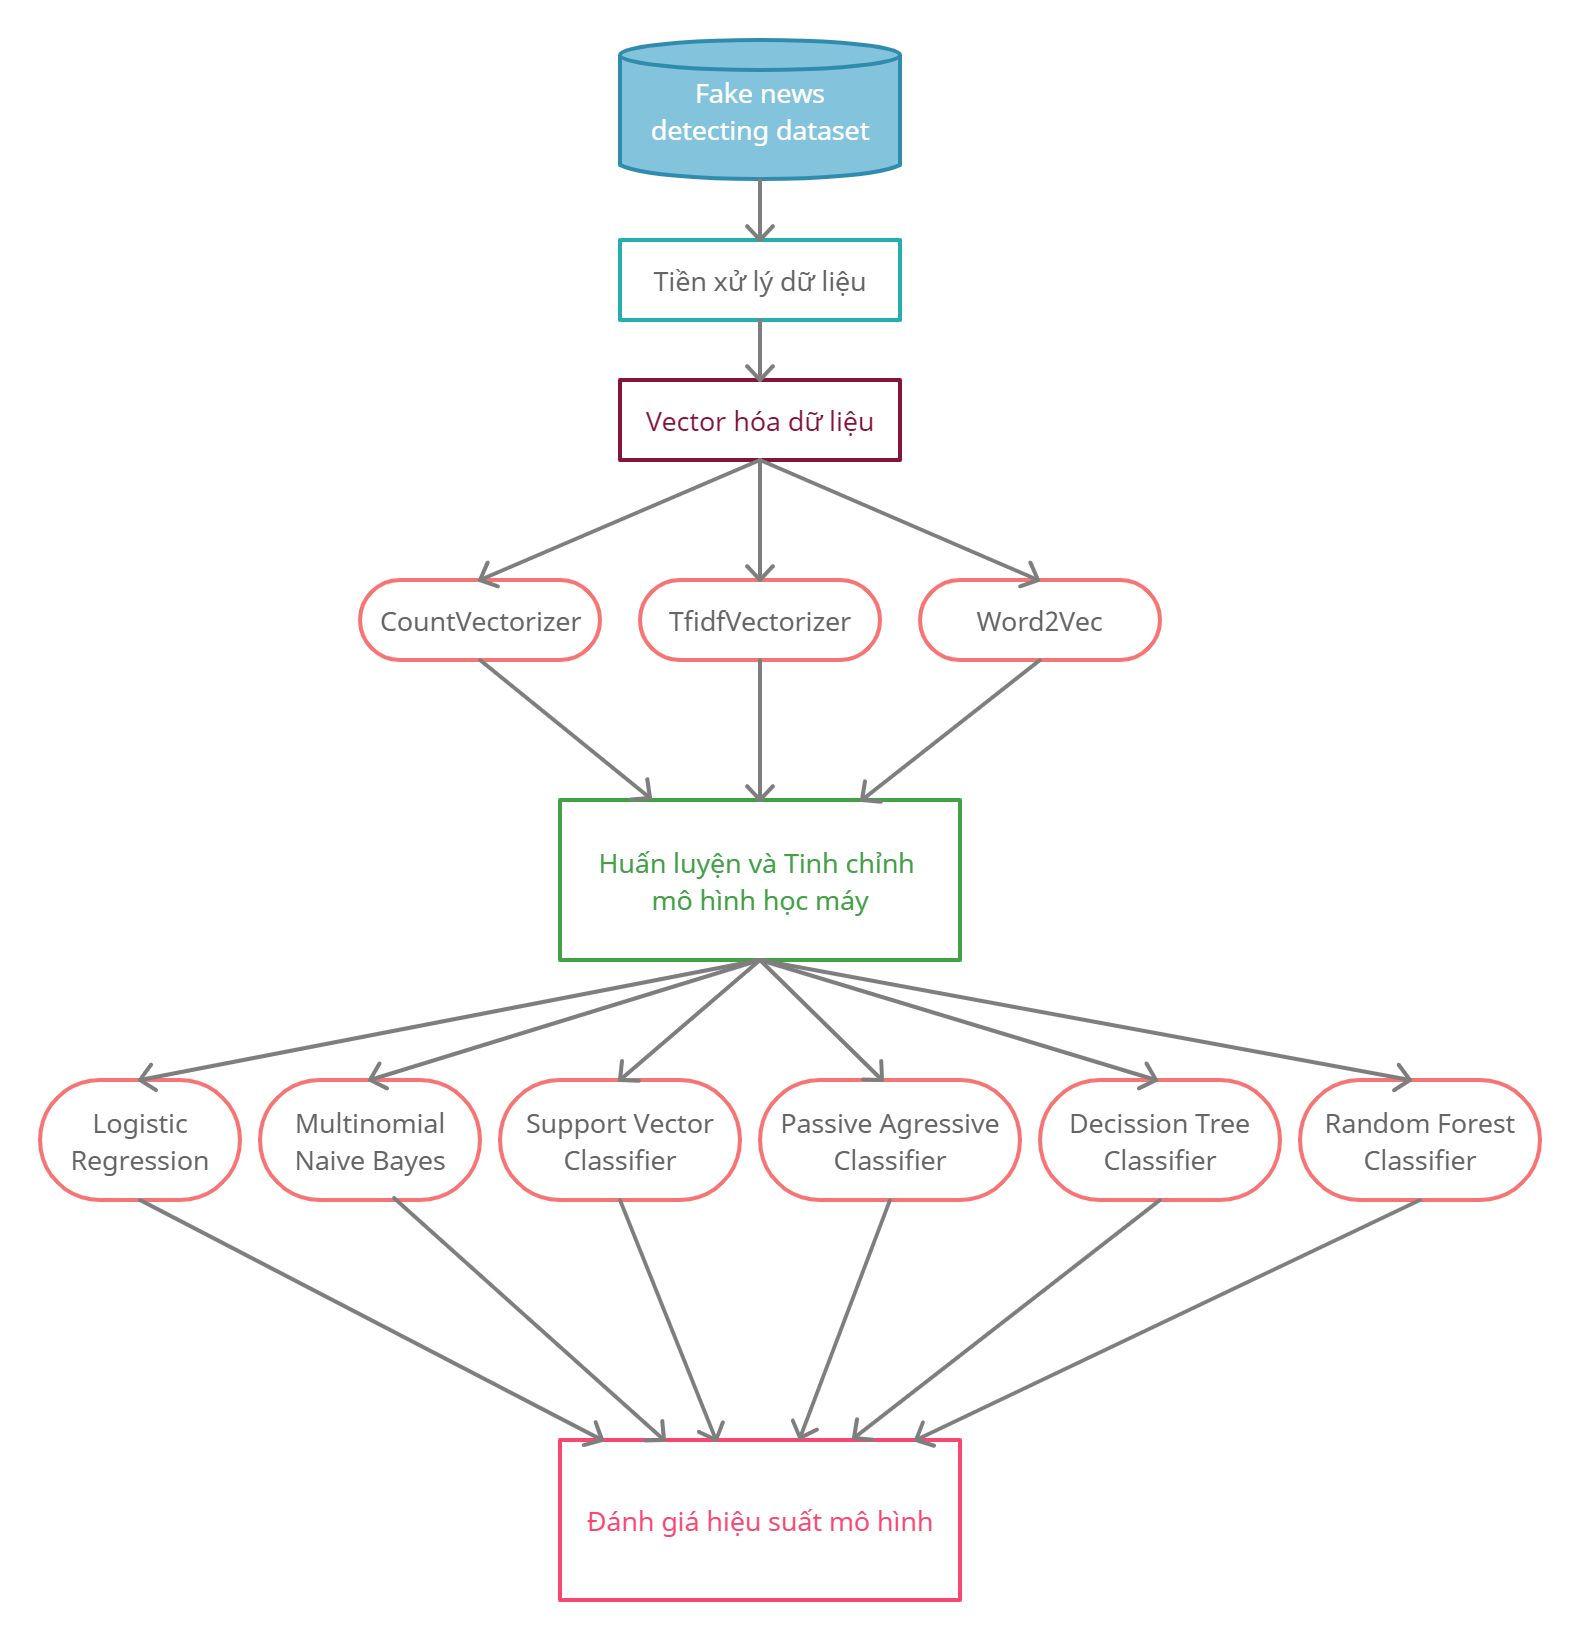
\includegraphics[width=0.88\columnwidth]{QuyTrinhHMTK}
		\end{center}
		\caption{Quy trình thực hiện bài toán Nhận diện tin giả}
	\end{figure}
	\section{Ứng dụng thực tiễn}
	Mã nguồn giải pháp cho bài toán Nhận diện tin giả có thể được tích hợp thành các module sử dụng trên nền tảng web hoặc trong các thiết bị quét văn bản,smartphone,... Qua đó có thể xác định, kiểm soát và ngăn chặn kịp thời tin giả từ các nguồn tin không chính thống lan ra cộng đồng, góp phần củng cố niềm tin của người dân và uy tín của các tổ chức xã hội.


\chapter{TỔNG QUAN VỀ BỘ DỮ LIỆU}

	

	\section{Giới thiệu chung về bộ dữ liệu}
	
	Bộ dữ liệu được chia sẻ bởi nhiều nguồn khác nhau trên nền tảng Kaggle. Thông qua tìm hiểu, chúng tôi tìm được bộ dữ liệu gốc của tác giả Raluca Chitic đăng tải vào ngày 23/05/2018. Vào thời điểm đó, tác giả được trích dẫn là chủ nhân của bộ dữ liệu trong một số bài báo nghiên cứu khoa học về đề tài này
	\footnote{ \href{https://www.researchgate.net/publication/339299161_Application_of_Supervised_Machine_Learning_Algorithms_to_Detect_Online_Fake_News}{\textit{Application of Supervised Machine Learning Algorithms to Detect Online Fake News}}}.
	
	Sau đây là thông tin của bộ dữ liệu.
	
	\begin{table}[h!]
	\renewcommand{\arraystretch}{1.5}
		\begin{center}
			
			\label{tab:table1}
			\begin{tabular}{|c|l|}
				\hline
				\multicolumn{1}{|c|}{\textbf{Thông tin}} & \multicolumn{1}{c|}{\textbf{Nội dung}}\\	
				\hline
				Tên bộ dữ liệu & Detecting Fake News Dataset\\
				\hline
				Nguồn dữ liệu & \url{https://www.kaggle.com/rchitic17/real-or-fake}\\
				\hline
				Kích thước bộ dữ liệu & 6335 điểm dữ liệu\\
				\hline
				Thông tin thuộc tính & 
				\begin{tabular}{l}
					4 thuộc tính. Trong đó:\\
						\tabitem Unnamed: ID dạng số ngẫu nhiên\\
						\tabitem title: Tiêu đề tin tức\\
						\tabitem text: Nội dung tin tức\\
						\tabitem label: Nhãn phân loại tin tức\\
				\end{tabular}\\ 
				\hline
				Ý nghĩa các nhãn & 
				\begin{tabular}{l}
					Có 2 nhãn "REAL" và "FAKE":\\
					\tabitem REAL: Đây là tin tức thật\\
					\tabitem FAKE: Đây là tin tức giả\\
				\end{tabular}\\
				\hline
				Thông tin Tác giả & Raluca Chitic, Đại học Luxembourg \\
				\hline
			\end{tabular}
			\caption{Thông tin bộ dữ liệu.}
		\end{center}
	\end{table}

	\section{Khám phá và trực quan bộ dữ liệu}
	
	\subsection{Thông tin mô tả bộ dữ liệu}
				\begin{figure}[H]
					\begin{center}
						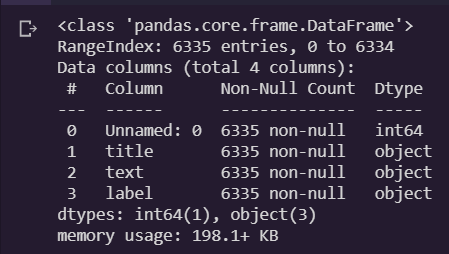
\includegraphics[width=0.78\columnwidth]{dfinfo}
					\end{center}
					\caption{Thông tin mô tả bộ dữ liệu}
				\end{figure}
				
	Chúng tôi sử dụng thư viện Pandas để đọc bộ dữ liệu từ file .csv và lưu  vào không gian làm việc dưới dạng Dataframe. Sau đó gọi thực hiện phương thức info() của Dataframe để lấy thông tin về bộ dữ liệu. 
	
	Bộ dữ liệu có 6335 điểm dữ liệu khác Null được đánh số từ 0 đến 6334 với đầy đủ 4 thuộc tính:
	\begin{itemize}
	\item \textbf{Unnamed: 0:} kiểu int
	\item \textbf{title:} kiểu object
	\item \textbf{text:} kiểu object
	\item \textbf{label:} kiểu object

	
	\end{itemize}
	\subsection{Phân bố nhãn của bộ dữ liệu}
			\begin{figure}[H]
				\begin{center}
					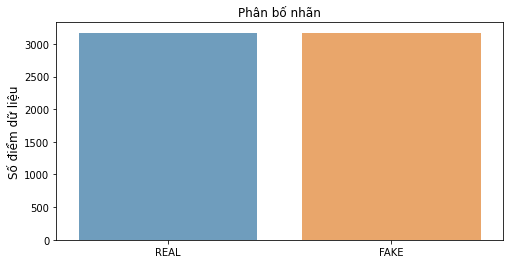
\includegraphics[width=0.8\columnwidth]{phanbonhan}
				\end{center}
				\caption{Phân bố nhãn của bộ dữ liệu}
			\end{figure}
			
	Số điểm dữ liệu có nhãn REAL: 3171
	
	Số điểm dữ liệu có nhãn FAKE: 3164
	
	Phân bố điểm dữ liệu trên hai nhãn là cân bằng. Sự cân bằng của dữ liệu giúp cho các mô hình phân lớp đạt độ chính xác cao và có tỉ lệ dự đoán đồng đều ở mỗi nhãn.

		\subsection{Những từ xuất hiện nhiều ở mỗi nhãn}
					\begin{figure}[H]
						\begin{center}
							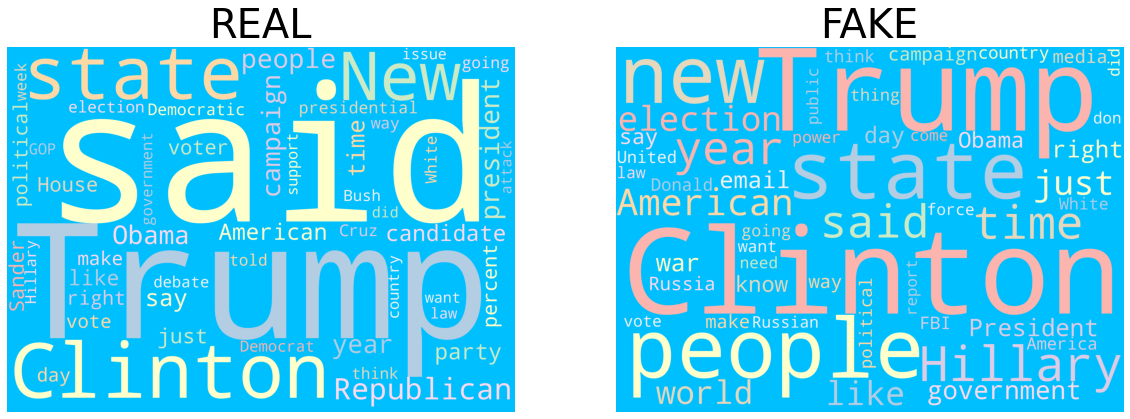
\includegraphics[width=0.9\columnwidth]{wordcloud}
						\end{center}
						\caption{Wordcloud những từ xuất hiện nhiều ở hai nhãn}
					\end{figure}
	Qua WordCloud có thể nhận thấy chủ đề tin tức xoay quanh tình hình chính trị và bầu cử tại Mỹ.
	
	Có một số từ xuất hiện nhiều ở hai nhãn như: `Trump', `Clinton', `said', `state',... Những từ này có thể gây nhiễu cho mô hình và ảnh hưởng đến kết quả dự đoán.
	\subsection{Phân bố độ dài nội dung}
	
	
	
	  \begin{figure}[!ht]
	  	
	    \centering
	    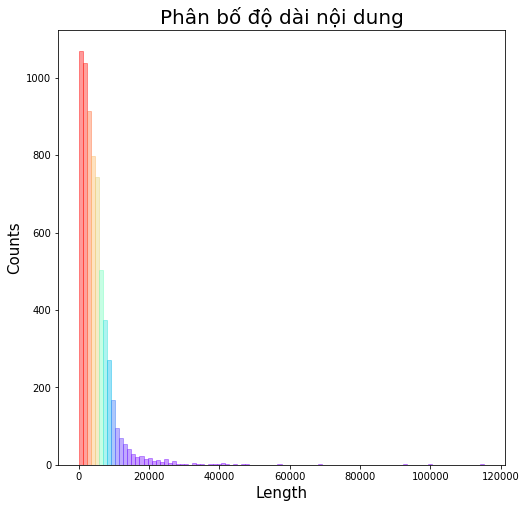
\includegraphics[width=0.71\columnwidth]{textlen}
	    \qquad
	    \footnotesize
	    \renewcommand{\arraystretch}{2.}
	    \begin{tabular}[b]{cc}\hline
	      \textbf{count} &  6335.00\\ \hline
          \textbf{mean} & 4707.25 \\ \hline
          \textbf{std} & 5090.96 \\ \hline
          \textbf{min} & 1.00 \\ \hline
          \textbf{25\%} & 1741.50 \\ \hline
          \textbf{50\%} & 3642.00 \\ \hline
          \textbf{75\%}  & 6192.00\\ \hline
          \textbf{max} & 115372.00\\ \hline 
          \vspace{2.5em} 
	    \end{tabular}
	    \caption{Phân bố và mô tả đồ dài nội dung tin tức}
	  \end{figure}
	
	
	
	  
	  
	  
	  
	  
	

\chapter{TIỀN XỬ LÝ VÀ VECTOR HÓA DỮ LIỆU}
	
	Trước khi thực hiện các bước tiền xử lý và vector hóa dữ liệu, chúng tôi sử dụng hàm train\_test\_split() hỗ trợ bởi thư viện scikit-learn để tiến hành phân chia tập train và tập test với tỉ lệ 75\% train - 25\% test. 
	
	Ở mỗi tập dữ liệu, chúng tôi bỏ đi cột \textit{Unnamed:0} và gộp nội dung 2 cột \textit{title} và \textit{text} lại để làm dữ liệu đầu vào. Đối với nhãn \textit{label}, chúng tôi ánh xạ giá trị dạng chuỗi ký tự về dạng nhị phân để mô hình có thể hoạt động hiệu quả.
		
	\[
	 label = \begin{cases}	    0 & \text{ nếu \textit{label} = FAKE} \\
	  1 & \text{ nếu \textit{label} = REAL}
	 \end{cases}
	\]
	
	\section{Tiền xử lý dữ liệu}
	
	Chúng tôi tiến hành thực hiện tuần tự các bước tiền xử lý sau trên cả hai tập train và test.
	
	\subsection {Loại bỏ ký tự số}
	
	Trong một mẩu tin tức hay một bài viết, những con số thường mang tính định lượng và không làm thay đổi ý nghĩa nội dung. Do đó, cách tốt nhất là loại bỏ chúng để hạn chế nhiễu trong dữ liệu.
	
	Chúng tôi loại bỏ các ký tự số bằng cách duyệt qua từng ký tự trong nội dung mẩu tin, sử dụng phương thức \textit{isdigit()} nhằm xác định ký tự số và thay thế chúng bằng ký tự rỗng. Sau bước này, dữ liệu đã được lọc bỏ các chữ số hoàn toàn.
	
	\subsection {Loại bỏ dấu câu và các ký tự đặc biệt}
	
	Ở bước này, chúng tôi tiến hành loại bỏ các ký tự không phải là chữ cái tiếng Anh, bao gồm các dấu ngắt câu và các ký tự đặc biệt sau:
	\begin{center}
	!"\#\$\%\&'()*+, -./:;<=>?@[\textbackslash]\textasciicircum \_ \`\{|\}$\sim$“”¨«»®´·º½¾¿¡§‘’£₤
	\end{center}
		
	Chúng tôi sử dụng hàm sub() trong module \textit{re} (Regular Expression) kết hợp với module \textit{string.punctuation} trong Python để tìm và loại bỏ đi những ký tự trên. 
	
	Sau khi thực hiện xong bước này, chúng tôi chuyển đổi nội dung của từng điểm dữ liệu thành danh sách các token bằng cách sử dụng phương thức \textit{split()} trong module \textit{re}, nhằm thực hiện các bước tiền xử lý tiếp theo.
	
	\subsection{Loại bỏ stop words}
	
	Stop words là những từ xuất hiện phổ biến nhưng không mang nhiều ý nghĩa. Trong tiếng Anh, một số từ là stop word như `a', `an', `the', `is'...  thường bị các công cụ tìm kiếm bỏ qua một phần hoặc hoàn toàn do chúng thường không liên quan đến nội dung mà văn bản đang đề cập.

 	Việc loại bỏ các stop words có thể mang lại một số hiệu quả nhất định. Kích thước dữ liệu có thể được cắt giảm mà không làm mất đi ý nghĩa của nội dung, giúp tiết kiệm tài nguyên tính toán và thời gian huấn luyện. Việc loại bỏ stop words cũng là cách hạn chế tác động của nhiễu đến mô hình, mô hình sẽ tập trung vào những phần nội dung mang nhiều ý nghĩa hơn để phân biệt tin thật và tin giả.
 	
 	Ở bước này, chúng tôi loại bỏ những token nằm trong danh sách stop words lấy từ module \textit{text.ENGLISH\_STOP\_WORDS} của thư viện scikit-learn.
 	
 	\subsection{Chuyển từ về dạng nguyên mẫu}
 	
 	Chúng tôi sử dụng hàm \textit{WordNetLemmatizer()} của bộ công cụ xử lý ngôn ngữ tự nhiên \textit{nltk toolkit} để thực hiện việc chuyển đổi các token về dạng nguyên mẫu. Việc chuyển đổi này nhằm  đơn giản hóa dữ liệu, giúp mô hình phân lớp tốt hơn.
 	
 	Sau bước này, tại mỗi điểm dữ liệu, chúng tôi gộp các token lại thành một văn bản hoàn chỉnh đã được tiền xử lý, sẵn sàng cho việc vector hóa để đưa vào các mô hình thực nghiệm.
 	
	\section{Trích xuất đặc trưng}
	
	\subsection{CountVectorizer}
	\textbf{Bag-of-Words}
	
	Mô hình máy học không thể làm việc trực tiếp với văn bản thô, do đó chúng ta sẽ đưa văn bản thô thành dạng vector số. 
	
	Bag-of-Words hay BoW là một kĩ thuật đơn giản, linh hoạt và khá hiệu quả trong xử lý ngôn ngữ tự nhiên. Mô hình BoW đơn giản là đưa các từ, các câu hay đoạn văn ở dạng text về vector có độ dài cố định mà mỗi phần tử là một số. Mỗi con số trong vector này là số lần xuất hiện của từ tương ứng trong văn bản đang xét. Trong mô hình này, văn bản được thể hiện dưới dạng túi (multiset) chứa các từ của nó, được gọi là "túi" vì mô hình chỉ quan tâm liệu từ đó xuất hiện bao nhiêu lần trong văn bản, nhưng không quan tâm đến ngữ pháp và trật tự các từ.
	
	\begin{figure}[H]
		\begin{center}
			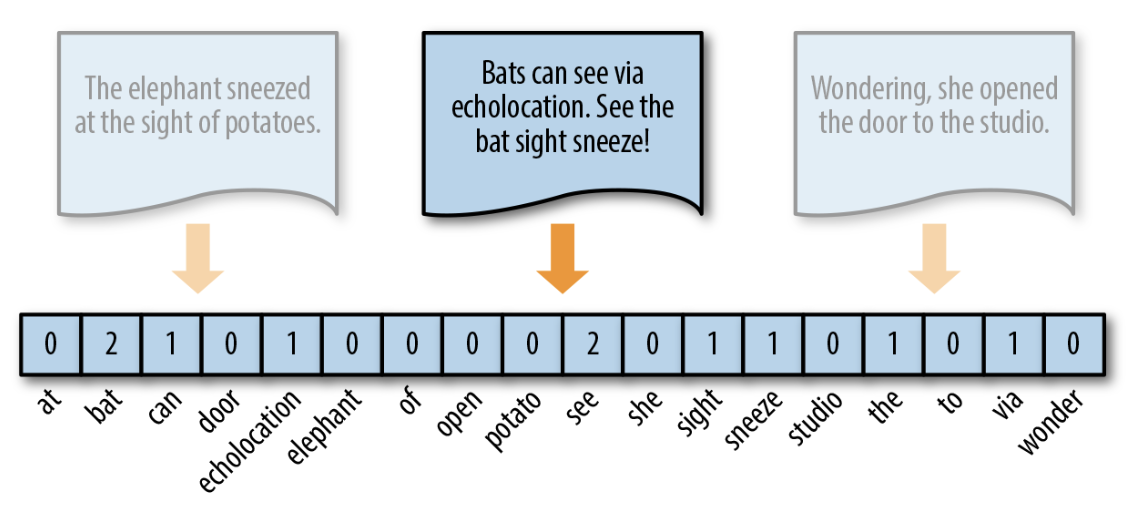
\includegraphics[width=0.8\columnwidth]{bow.png}
		\end{center}
		\caption{Ví dụ về Bag-of-Words}
	\end{figure}
	Ở ví dụ trên, dựa trên 3 văn bản, ta có danh sách tập các từ được sử dụng, danh sách này còn được gọi là từ điển (vocabulary) với 18 từ. Sau khi áp dụng BoW, ta có vector đặc trưng của văn bản thứ hai có số chiều bằng 18, với mỗi phần tử là số lần xuất hiện của từ tương ứng trong văn bản.
	
	\textbf{N-Grams}
	
	Như đề cập ở trên, mô hình BoW chỉ quan tâm số lần xuất hiện của từ, và không coi trọng trật tự của các từ hay cụm từ. Ví dụ một dữ liệu gồm 2 câu văn bản sau đây:
	
	\hspace{1cm} Văn bản 1: "hôm nay trời nắng"
	
	\hspace{1cm} Văn bản 2: "nắng trời nay hôm"
	
	Văn bản 1 là một câu đúng ngữ pháp và diễn đạt trôi chảy hơn các từ có thứ tự ngẫu nhiên ở văn bản 2. Tuy vậy, BoW của cả 2 văn bản là như nhau, vì thế mô hình sẽ đánh giá không tốt ở dữ liệu này.
	
	Thay vào đó, mô hình n-grams có thể lưu trữ thông tin thứ tự các từ này:
	\begin{itemize}
		\item Kích thước n = 1 được gọi là "Unigram": tính tần suất xuất hiện của một từ.
		\item Kích thước n = 2 gọi là "Bigram": tính tần suất xuất hiện của một từ nếu biết 1 từ đứng cạnh nó.
		\item Kích thước n = 3 là "Trigram": tính tần suất xuất hiện của một từ nếu biết 2 từ đứng cạnh nó.
	\end{itemize}
	Và tương tự vậy, n càng lớn thì số trường hợp càng lớn, tuy cho độ chính xác của tần suất xuất hiện của từ cao nhưng độ phức tạp sẽ khó hơn. 
	\begin{figure}[H]
		\begin{center}
			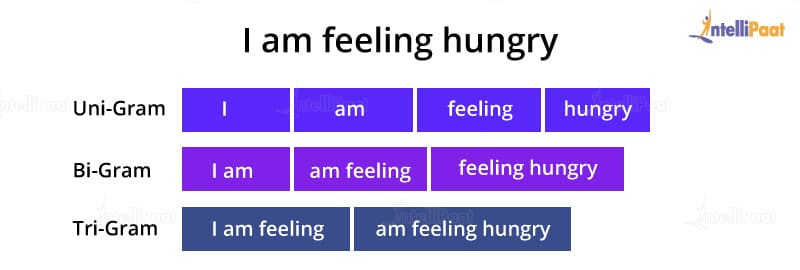
\includegraphics[width=0.8\columnwidth]{ngrams.jpg}
		\end{center}
		\caption{Ví dụ về N-Grams}
	\end{figure}
	
	
	\textbf{Triển khai mô hình Bag-of-Words với CountVectorizer}
	
	Chúng tôi sử dụng CountVectorizer của thư viện sklearn để chuyến hoá văn bản thành các vector đặc trưng với các tham số sau:
	\begin{itemize}
		\item ngram\_range=(1,2): tính cho Unigram và Bigram.
		\item tokenizer=tokenize: tách câu thành từ mà vẫn giữ nguyên bước tiền xử lý và n-grams.
		\item token\_pattern = None: Ở bước tiền xử lý chúng tôi đã loại bỏ các ký tự đặc biệt, do đó tham số này sẽ có giá trị là None.
		\item analyzer='word': đơn vị tính là từ.
		\item min\_df=5: bỏ qua các từ hoặc cụm từ chỉ xuất hiện dưới 5 văn bản.
		\item max\_df=0.9: bỏ qua các từ hoặc cụm từ xuất hiện trong hơn 90\% tổng số văn bản.
		\item strip\_accents='unicode': loại bỏ các ký tự Unicode
	\end{itemize}
	
	Trong bài toán thực tế, tập các từ được sử dụng (vocabulary) có rất nhiều từ, như thế vector đặc trưng thu được sẽ rất dài. Và có rất nhiều từ trong tập vocabulary không xuất hiện trong văn bản, như vậy các vector đặc trưng thu được có nhiều phần tử bằng 0 (vector này được gọi là sparse vector) chiếm nhiều không gian lưu trữ không mong muốn. Hoặc một vấn đề có thể ta gặp phải là có những từ hiếm không nằm trong tập vocabulary và từ hiếm đôi khi mang lại thông tin quan trọng mà ta có thể bỏ qua. Có một phương pháp cải tiến khắc phục nhược điểm của BoW có tên là TFIDF. TFIDF sẽ chú trọng trong việc xác định độ quan trọng của một từ trong văn bản dựa trên toàn bộ tập các văn bản. 
	
	\subsection{TF-IDF}
	

			
			TF-IDF viết tắt của Term Frequency - Inverse Document Frequency, là một hướng tiếp cận khác của mô hình Bag-of-Words. TF-IDF của một từ (cụm từ) hay token là một giá trị thể hiện mức độ quan trọng của từ (cụm từ) này trong một văn bản (document), mà bản thân văn bản này đang nằm trong một tập hợp các văn bản (corpus). Từ nào càng xuất hiện nhiều trong một văn bản và đồng thời xuất hiện trong các văn bản khác thì nó mang tính đặc trưng cao cho văn bản đó.
	
			\textbf{Công thức tính TF-IDF}
			 \paragraph{TF - Term Frequency}
			là giá trị thể hiện tần suất xuất hiện của một từ trong văn bản. Nếu từ đó xuất hiện càng nhiều thì trọng số càng cao. Công thức tính bằng thương của số lần xuất hiện 1 từ trong văn bản và số lần xuất hiện nhiều nhất của một từ bất kỳ trong văn bản đó. Giá trị này sẽ thuộc khoảng [0, 1].
			\begin{equation}
				\operatorname{tf}(t, d)= \frac{\operatorname{f}(t,d)}{max\{\operatorname{f}(w,d) : w \in d \}}
			\end{equation}
		 	\begin{itemize}
		 		\item \textbf{$\operatorname{f}(t,d)$} – số lần xuất hiện từ \textbf{t} trong văn bản \textbf{d}
		 		\item \textbf{$max\{\operatorname{f}(w,d) : w \in d \}$} – số lần xuất hiện nhiều nhất của một từ bất kỳ trong văn bản.
		 	\end{itemize}
		 	
	 		 Nếu chỉ xét theo tần suất xuất hiện của từng từ thì việc phân loại văn bản rất có thể cho kết quả sai dẫn tỷ lệ chính xác sẽ thấp. Giải pháp khắc phục cho điều này là sử dụng phương pháp thống kê \textbf{TF-IDF}.
	 		\paragraph{IDF – Inverse Document Frequency} là tần suất xuất hiện của một từ trong tập văn bản. Mục đích tính IDF là để giảm giá trị của những từ phổ biến. 
	 		\begin{equation}
	 			\operatorname{idf}(t,D) = \log\frac{\lvert D \rvert}{\lvert \{ d \in D : t \in d \} \rvert}
	 		\end{equation}
	 		\begin{itemize}
	 			\item $\lvert D \rvert$ – tổng số văn bản trong tập \textbf{D}
	 			\item $\lvert \{ d \in D : t \in d \} \rvert$ – số văn bản chứa từ nhất định, với điều kiện \textbf{t} xuất hiện trong văn bản \textbf{d}. Nếu từ đó không xuất hiện ở bất cứ 1 văn bản nào trong tập thì mẫu số sẽ bằng 0. Do đó, phép chia cho không không hợp lệ, vì thế người ta thường thay mẫu thức là $1 + \lvert \{ d \in D : t \in d \} \rvert$
	 		\end{itemize}
	
	 		\paragraph{Giá trị TF-IDF}
			\begin{equation}
			\operatorname{tfidf}(t,d,D) = \operatorname{tf}(t,d) \times \operatorname{idf}(t,D)
			\end{equation}
			
			Trong ngôn ngữ luôn có những từ xuất hiện thường xuyên hơn. Chính vì vậy  ta cần có một phương pháp để làm mịn đường cong tần số trên hay cân bằng mức độ quan trọng giữa các từ. TF-IDF cũng được sử dụng để lọc những từ stopwords trong các bài toán như tóm tắt văn bản và phân loại văn bản.
			
			Để chuyển văn bản đầu vào thành các vector TFIDF, chúng tôi sử dụng công cụ \textit{TfidfVectorizer} của thư viện sklearn với các tham số sau:
			
			\begin{itemize}
			\item ngram\_range = (1,2): tính TFIDF cho Unigram và Bigram.
			\item analyzer = `word' : đơn vị tính TFIDF là từ.
			\item min\_df = 5: bỏ qua các từ hoặc cụm từ chỉ xuất hiện trong dưới 5 văn bản.
			\item max\_df = 0.9: bỏ qua các từ hoặc cụm từ xuất hiện trong hơn 90\% tổng số văn bản.
			\item strip\_accent = `unicode': loại bỏ các ký tự Unicode.
			\item sublinear\_tf = True: Thay tf bằng 1+ $\log$(tf)
			\end{itemize}
			
			
	\subsection{Word2Vec}
	
	Word2Vec là một trong những mô hình đầu tiên về Word Embedding sử dụng Neural Network và được áp dụng phổ biến trong lĩnh vực Xử lý Ngôn ngữ tự nhiên. Word2Vec có khả năng vector hóa văn bản, từ hay cụm từ về dạng vector số dựa trên tập các từ chính và các từ ngữ cảnh, từ đó làm đầu vào cho việc huấn luyện các mô hình Học máy hoặc các mô hình Học sâu.
	
	Với tính chất của Word Embedding, mô hình Word2Vec đảm bảo rằng các từ tương tự nhau sẽ có giá trị vector gần giống nhau. Ví dụ như vector của King, Queen hoặc vector của Man, Woman là tương tự nhau và đặc biệt ta có King – Man + Woman ≈ Queen.
	
	\begin{figure}[H]
		\begin{center}
			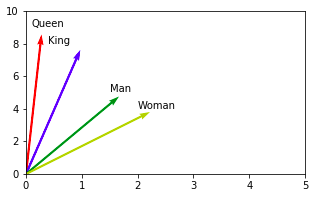
\includegraphics[width=0.8\columnwidth]{wordembedding}
		\end{center}
		\caption{Mô tả các vector Word Embedding Queen, King, Man, Woman}
	\end{figure}

	
	Về mặt toán học, thực chất Word2Vec là việc ánh xạ từ một tập các từ vựng (vocabulary) sang một không gian vector, mỗi vector được biểu diễn bởi n số thực. Mỗi từ ứng với 1 vector cố định. Sau quá trình huấn luyện mô hình bằng thuật toán backpropagation, trọng số các vector của từng từ được cập nhật liên tục. Từ đó, ta có thể thực hiện tính toán bằng các khoảng cách quen thuộc như euclide, cosine, manhattan,... Những từ càng "gần" nhau về mặt khoảng cách thường là các từ hay xuất hiện cùng nhau trong văn cảnh, các từ đồng nghĩa, các từ thuộc cùng 1 trường từ vựng,
	
	Mô hình chung của Word2Vec dựa trên 1 mạng neural khá đơn giản. Gọi V là tập các tất cả các từ hay vocabulary với n từ khác nhau. Layer input biểu diễn dưới dạng one-hot encoding với n node đại diện cho n từ trong vocabulary. Activation function (hàm kích hoạt) chỉ có tại layer cuối là softmax function, loss function là cross entropy loss, tương tự như cách biểu diễn mô hình của các bài toán classification thông thường. Ở giữa hai layer input và output là một layer trung gian với size = k, chính là vector sẽ được sử dụng để biểu diễn các từ sau khi huấn luyện mô hình.
	
	\begin{figure}[H]
		\begin{center}
			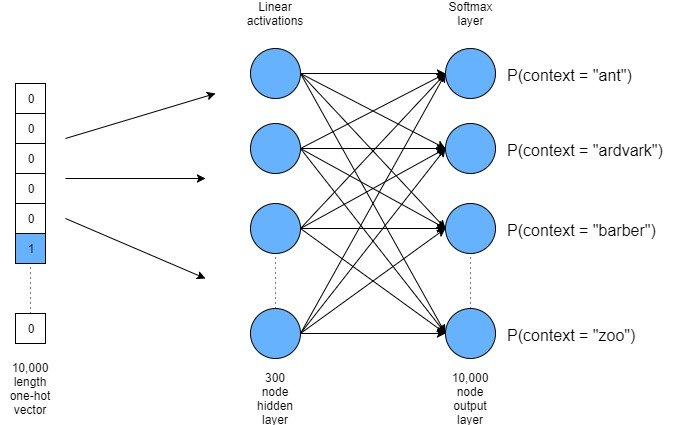
\includegraphics[width=0.7\columnwidth]{w2v_ex}
		\end{center}
		\caption{Ví dụ về mô hình Word2Vec}
	\end{figure}
	
	Trong Word2Vec có hai khái niệm quan trọng là \textit{center word} và \textit{context words}.
	Hiểu đơn giản là ta sẽ sử dụng từ ở giữa (\textit{center word}) cùng với các từ xung quanh nó (\textit{context words}) để mô hình thông qua đó để tiến hành huấn luyện. Dựa trên đó, mô hình Word2Vec có hai cách tiếp cận chính:
	
	\begin{itemize}
	\item \textbf{CBOW (Continuous Bag of Words)} 
	
	\begin{figure}[H]
		\begin{center}
			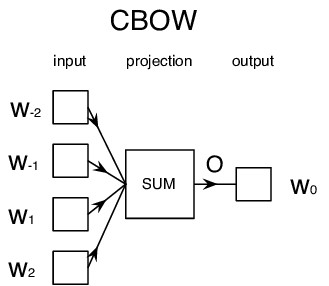
\includegraphics[width=0.32\columnwidth]{cbow}
		\end{center}
		\caption{Mô hình CBOW}
	\end{figure}
	Ý tưởng chính của CBOW là dựa vào các \textit{context word} để dự đoán \textit{center word}. CBOW có điểm thuận lợi là huấn luyện mô hình nhanh hơn so với mô hình Skip-gram, thường cho kết quả tốt hơn với frequency words (hay các từ thường xuất hiện trong ngữ cảnh)
	\item \textbf{Skip-gram}
	
	\begin{figure}[H]
		\begin{center}
			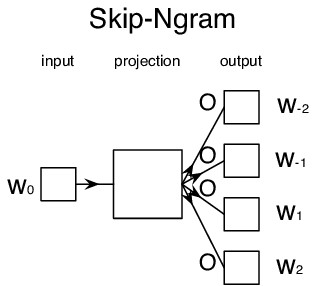
\includegraphics[width=0.32\columnwidth]{skipgram}
		\end{center}
		\caption{Mô hình Skip-gram}
	\end{figure}
		
	Mô hình Skip-gram thì ngược lại với CBOW, dùng \textit{center word} để dự đoán các từ xung quanh. Skip-gram huấn luyện chậm hơn. Thường làm việc khá tốt với các tập data nhỏ, đặc biệt do đặc trưng của mô hình nên khả năng vector hóa cho các từ ít xuất hiện tốt hơn CBOW.
	
	\end{itemize}
	
	Trong đồ án này, chúng tôi sử dụng mô hình Word2Vec đã được huấn luyện sẵn trên bộ Google News Vector kích thước 300 chiều với khoảng 3 triệu từ và cụm từ. Thông thường việc huấn luyện trên có thể mất đến hàng giờ, tuy nhiên mô hình đã có sẵn nên việc tải và load lên Google Colab với thư viện Gensim chỉ mất vài phút. 
	
	Sau khi đã có mô hình, chúng tôi thực hiện việc chuyển đổi dữ liệu dạng văn bản về dạng vector số thực bằng cách lấy trung bình của các giá trị vector từ pretrain model ứng với từng từ trong mỗi văn bản. Một cách chi tiết hơn, chúng tôi xét mỗi từ trong một văn bản, nếu một từ có trong bộ pretrain model Google News Vector 300, mô hình sẽ trả về một vector số thực 300 chiều ứng với từ đó. Trung bình của các vector số thực này sẽ là một vector 300 chiều đại diện cho điểm dữ liệu (văn bản).
	
	Như vậy ma trận thu được sau khi chuyển đổi sẽ có số chiều là n x 300, với n là kích thước của tập huấn luyện hay tập kiểm thử.
	
	Để không gặp lỗi nhận giá trị âm khi huấn luyện một số mô hình như MultinomialNB, chúng tôi sử dụng công cụ \textit{MinmaxScaler} của thư viện scikit-learn để ánh xạ tập số thực về tập giá trị nằm trong khoảng (0,1)

\chapter{HUẤN LUYỆN VÀ TINH CHỈNH CÁC MÔ HÌNH HỌC MÁY}
	\section{Cơ sở lý thuyết}
		\subsection{Logistic Regression}
			Phương pháp Logistic Regression là một mô hình hồi quy được sử dụng phổ biến cho bài toán phân lớp nhị phân.

			Mô hình hoạt động dựa trên hàm sigmoid với đường cong chữ S đặc trưng, dùng để dự đoán xác suất xảy ra hay không xảy ra của một nhãn nào đó.
			
			\begin{figure}[H]
				\begin{center}
					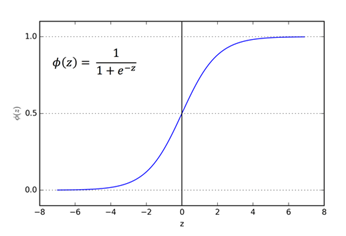
\includegraphics[width=0.8\columnwidth]{Picture1}
				\end{center}
				\caption{Đồ thị hàm sigmoid}
			\end{figure}
			
			Đầu ra của bài toán logistic regression với dữ liệu đầu vào \textbf{x} và vector hệ số \textbf{w} thường viết chung dưới dạng:
			
			\begin{center}
				$f(x) = \dfrac{1}{1+e^{-\textbf{w}^T\textbf{x}}}$
			\end{center}
			
			Sau khi tìm được mô hình, việc xác định class \textbf{y} cho một điểm dữ liệu \textbf{x} được xác định bằng việc so sánh hai biểu thức xác suất:
			
			\begin{center}
				$P(y=1|\textbf{x};\textbf{w}); P(y=0|\textbf{x};\textbf{w})$
			\end{center}
			
			Vì tổng hai biểu thức này luôn bằng 1 nên một cách gọn hơn, ta cần xác định xem $P(y=1|\textbf{x};\textbf{w})$ có lớn hơn 0.5 hay không. Nếu lớn hơn 0.5, ta kết luận điểm dữ liệu thuộc class 1, ngược lại thì điểm dữ liệu thuộc class 0.
			
			\textbf{Công cụ sử dụng:} Hàm \textit{LogisticRegression} trong module \textit{linear\_model} của thư viện scikit-learn
			
		\subsection{Multinomial Naive Bayes}
			Bộ phân lớp Naive Bayes (NBC) thường được sử dụng trong các bài toán phân loại văn bản, với thời gian train và test rất nhanh. Điều này có được do giả sử về tính độc lập giữa các thành phần, nếu biết class. Nếu giả sử về tính độc lập được thoả mãn (dựa vào bản chất của dữ liệu), NBC được cho là cho kết quả tốt hơn so với SVM và Logistic Regression khi có ít dữ liệu training.

			NBC có thể hoạt động với các feature vector mà một phần là liên tục (sử dụng Gaussian Naive Bayes), phần còn lại ở dạng rời rạc (sử dụng Multinomial hoặc Bernoulli).

			Mô hình Multinomial Naive Bayes chủ yếu được sử dụng trong bài toán phân loại văn bản mà vector đặc trưng được xây dựng dựa trên ý tưởng Bag of words (BoW). Lúc này, mỗi văn bản được biểu diễn bởi một vector có độ dài d (là số từ trong văn bản). Giá trị của thành phần thứ i trong mỗi vector là số lần từ thứ i xuất hiện trong văn bản đó.

			Khi đó $p(\textbf{x}_i|c)$ tỉ lệ với tần suất từ thứ i (hay đặc trưng thứ i trong trường hợp tổng quát) xuất hiện trong các văn bản có class c. Giá trị này được tính bởi công thức:
			
			\begin{center}
				$\lambda_{ci} = p(\textbf{x}_i|c) = \cfrac{N_{ci}}{N_c}$    $(*)$
			\end{center}
			
			Trong đó:
			
			\begin{itemize}
				\item $N_{ci}$ là tổng số lần từ thứ i xuất hiện trong các văn bản của class c, nó được tính là tổng của tất cả các thành phần thứ i của các feature vectors ứng với class c.
				\item $N_c$ là tổng số từ (kể cả lặp) xuất hiện trong class c. Nói cách khác, nó bằng tổng độ dài của toàn bộ các văn bản thuộc vào class c.
			\end{itemize}
			
			Cách tính này có một hạn chế là nếu có một từ mới chưa bao giờ xuất hiện trong nhãn c thì biểu thức $(*)$ sẽ bằng 0. Để giải quyết việc này, một kỹ thuật được gọi là làm mềm Laplace (Laplace Smoothing) được áp dụng:
			
			\begin{center}
				$\hat{\lambda}=\cfrac{N_{ci}+\alpha}{N_c+d\alpha}$
			\end{center}
			
			Với $\alpha$ là một số dương (thường bằng 1) để tránh trường hợp tử số bằng 0. Mẫu số được cộng với $d\alpha$ để đảm bảo tổng xác suất bằng 1.
			
			Như vậy, mỗi nhãn c được mô tả bằng một bộ các số dương có tổng bằng 1:
			
			\begin{center}
				$\hat{\lambda_c}=\hat{\lambda}c1,..., \hat{\lambda}cd$
			\end{center}
			
		\textbf{Công cụ sử dụng:} Hàm \textit{MultinomialNB} trong module \textit{naive\_bayes} của thư viện scikit-learn
		
		\subsection{Support Vector Machine}
		Mục tiêu của SVM là tìm ra một siêu phẳng trong không gian N chiều (ứng với N đặc trưng) chia dữ liệu thành hai phần tương ứng với lớp của chúng. Nói theo ngôn ngữ của đại số tuyến tính, siêu phẳng này phải có lề cực đại và phân chia hai bao lồi và cách đều chúng.
		
			\begin{figure}[H]
			\begin{center}
		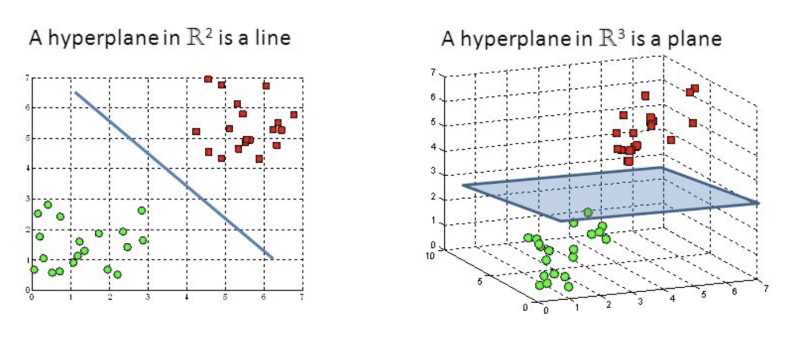
\includegraphics[width=0.68\columnwidth]{SVM_hyperplane}
			\end{center}
		\caption{Siêu phẳng tạo ra một biên giới phân chia 2 lớp của dữ liệu}
			\end{figure}		
		
		\textbf{Biên (hay lề - Margin)}
		
		Là khoảng cách giữa siêu phẳng đến 2 điểm dữ liệu gần	nhất tương ứng với 2 phân lớp. Một cách trực quan, đường thẳng phân tách 2 tập nhãn là tốt nhất nếu như nó không quá gần một tập nào đó, nghĩa là độ rộng biên M là cực đại.
		
			\begin{figure}[H]
			\begin{center}
				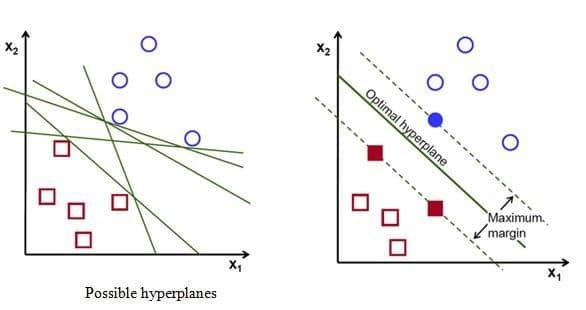
\includegraphics[width=0.68\columnwidth]{SVM_maxmargin}
			\end{center}
			\caption{Siêu phẳng tối ưu có lề cực đại}
			\end{figure}
		
		\textbf{Vector hỗ trợ}
		
		Phía trên chính là ý tưởng của phương pháp SVM. Bên cạnh đó, các vector hỗ trợ - là các điểm dữ liệu nằm trên hoặc gần nhất với siêu phẳng, chúng ảnh hưởng đến vị trí và hướng của siêu phẳng. Các vector này được sử dụng để tối ưu hóa lề và nếu xóa các điểm này, vị trí của siêu phẳng sẽ thay đổi. Một điểm lưu ý nữa đó là các vector hỗ trợ phải cách đều siêu phẳng.
		
		SVM giải quyết vấn đề overfitting rất tốt, là phương pháp phân lớp nhanh, có hiệu suất tổng hợp tốt và có hiệu suất tính toán cao.
		
		\textbf{Tham số C}
		
		Tham số C được gọi là "siêu tham số" (hyperparameter). Tham số C cho biết mức độ tối ưu hoá SVM để giảm thiểu phân lớp sai (misclassification) đối với điểm dữ liệu mới đi vào. Nếu mô hình SVM quá khớp (overfitting), ta có thể điều chỉnh giảm tham số C (khi đó độ rộng biên sẽ tăng lên) và ngược lại, tham số C càng lớn thì độ rộng biên càng hẹp.
		
		\textbf{Tham số gamma}
		
		Gamma là một siêu tham số được sử dụng với SVM phi tuyến tính. Một trong những nhân phi tuyến tính được sử dụng phổ biến nhất là hàm cơ sở xuyên tâm (RBF). Tham số gamma của RBF kiểm soát khoảng cách ảnh hưởng của một điểm đào tạo duy nhất.
		
		Giá trị thấp của gamma cho thấy bán kính tương tự lớn dẫn đến nhiều điểm được nhóm lại với nhau. Đối với các giá trị cao của gamma, các điểm cần phải rất gần nhau để được xem xét trong cùng một nhóm (hoặc lớp). Do đó, các mô hình có giá trị gamma rất lớn có xu hướng quá mức.
		
		\textbf{Thủ thuật Kernel}
		
		Một kernel là một hàm ánh xạ dữ liệu từ không gian ít chiều hơn sang không gian nhiều chiều hơn, từ đó ta tìm được siêu phẳng phân tách dữ liệu. Các kiểu kernel:
		\begin{itemize}
			\item Tuyến tính
			\item Đa thức
			\item RBF
			\item sigmoid
		\end{itemize}
		
		\textbf{Công cụ sử dụng:} Hàm \textit{SVC} trong module \textit{svm} của thư viện scikit-learn.
		
		\subsection{Thuật toán Passive Aggressive}
		
		Thuật toán Passive Aggressive là một phân nhóm các thuật toán Online learning dùng cho hai bài toán Hồi quy và Phân loại. Thuật toán này được giới thiệu lần đầu vào năm 2006, bởi Koby Crammer cùng các cộng sự tại Đại học Hebrew của Jerusalem, Israel.
		
		Trong các thuật toán Online learning, tập huấn luyện được chia nhỏ và đưa vào mô hình một cách tuần tự, và dựa trên mỗi nhóm nhỏ dữ liệu này, các mô hình Học máy sẽ 'học' và tự điều chỉnh. Cơ chế này rất hữu ích trong trường hợp kích thước dữ liệu quá lớn khiến cho việc huấn luyện trên toàn bộ tâp dữ liệu gặp nhiều khó khăn. Điển hình là bài toán nhận diện tin giả trên các nền tảng mạng xã hội như Twitter, Facebook,... nơi mà dữ liệu được sinh ra liên tục và nhanh chóng đạt kích thước khổng lồ. Trong trường hợp đó, các thuật toán Online Learning được xem là lý tưởng.
		
		
		\begin{figure}[H]
			\begin{center}
				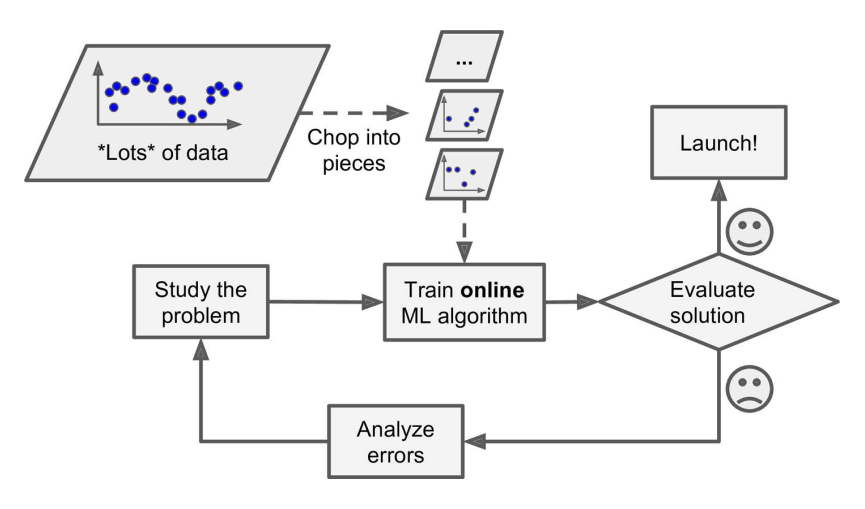
\includegraphics[width=0.8\columnwidth]{onl_learn}
			\end{center}
			\caption{Thuật toán Online Learning cho việc xử lý dữ liệu lớn}
		\end{figure}
		
		Nội dung của thuật toán Passive Aggressive có thể được hiểu một cách ngắn gọn từ tên của nó:

		\begin{itemize}
		\item \textbf{Passive:} Nếu dự đoán điểm dữ liệu chính xác thì mô hình được giữ lại và không điều chỉnh (điểm dữ liệu không đủ khiến mô hình phải điều chỉnh).
		\item \textbf{Aggressive:} Nếu dự đoán sai, mô hình phải thực hiện các điều chỉnh. Trong số đó sẽ có những điều chỉnh làm cho mô hình dự đoán đúng điểm dữ liệu đó.
		\end{itemize}
		
		Thư viện scikit-learn cũng hỗ trợ thuật toán Passive Aggressive thông qua hai hàm PassiveAggressiveRegressor() và PassiveAggressiveClassifier() trong module linear\_model.
		Ở đồ án này, mô hình PassiveAgressiveClassifier() được sử dụng với các tham số quan trọng sau:
		\begin{itemize}
		\item \textbf{C:} là độ chính quy hóa của mô hình. C càng lớn thì độ Aggressive của mô hình càng cao.
		\item \textbf{max\_iter:} số lần lặp tối đa của mô hình trên tập dữ liệu huấn luyện. Giá tri mặc định là 1000.
		\item \textbf{tol:} tiêu chuẩn dừng vòng lặp của mô hình. Giá trị mặc định là 0.001.
		\item \textbf{early\_stopping:} Nếu nhận giá trị True, mô hình sẽ tự động dừng huấn luyện nếu kết quả trên tập thẩm định không cải thiện.
		\end{itemize}
		
		\textbf{Công cụ sử dụng:} Hàm \textit{PassiveAgressiveClassifier} trong module \textit{linear\_model} của thư viện scikit-learn
				
		\subsection{Decision Tree}
		Decision Tree (cây quyết định) là mô hình thuộc nhóm thuật toán học máy học có giám sát (Supervised Learning). Mô hình cây quyết định cho biết giá trị của một biến mục tiêu thuộc lớp nào bằng cách dựa vào các giá trị của một tập các biến dự đoán, hay tập các câu hỏi.
		
		Cây quyết định có dạng cấu trúc cây, bao gồm: nút gốc (root node), nút quyết định (decision node) và nút lá (leaf node).
		
		\begin{itemize}
		\item \textbf{Nút gốc:} Là nút đầu tiên trong cấu trúc cây, thường nằm trên cùng, các nút khác trong cấu trúc cây bắt nguồn từ nút gốc.
		\item \textbf{Nút quyết định:} Là nút có một hoặc nhiều phân nhánh tới nút con, nút này tương ứng với biến dự đoán.
		\item \textbf{Nút lá:} Là giá trị dự đoán của biến mục tiêu.
		\item Nhánh nối giữa một nút và nút con thể hiện giá trị cụ thể cho biến đó.
		\end{itemize}
		
		Quy tắc để có được giá trị dự đoán cụ thể là biểu diễn đường đi từ nút gốc đi xuyên qua cây theo các nhánh đến nút lá. Từ đó, cây quyết định sẽ sinh ra các luật để dự đoán lớp của các dữ liệu chưa biết. Giải bài toán phân lớp dựa trên mô hình cây quyết định chính là xây dựng một cây quyết định.
		
		Hai thuật toán xây dựng cây quyết định phổ biến là CART và ID3.
		
		\textbf{Thuật toán CART sử dụng độ đo Gini}
		
		Gini index là chỉ số mức độ nhiễu loạn thông tin hay sự khác biệt về giá trị lớp của mỗi điểm dữ liệu trong một tập hợp con. Gini index cho phép đánh giá sự tối ưu của từng cách phân nhánh thông qua xác định mức độ purity của từng nút trong mô hình cây quyết định.
		
		Công thức tổng quát hệ số Gini:
		\begin{equation}
			GINI(t) = 1 - \sum_{j} [p(j|t)]^2
		\end{equation}
	
		Trong đó, t là một nút bất kỳ có chứa các điểm dữ liệu mang lớp j của biến mục tiêu và p là xác suất để một điểm dữ liệu trong t có lớp j, nếu tất cả các điểm dữ liệu đều mang lớp j, lúc này p = 1 và hệ số Gini sẽ bằng 0, khi đó nút được công nhận là pure node
		
		\textbf{Thuật toán ID3 sử dụng độ đo Entropy}
		
		Công thức tổng quát Entropy:
		\begin{equation}
			Entropy(t) = - \sum_{j} [p(j|t)]^2 \times log_{2}[p(j|t)] 
		\end{equation}
	
		Khi xác suất p càng lớn thì $log_{2}[p(j|t)]$ sẽ mang giá trị âm tiến tới 0, nhân với giá trị âm xác suất thì công thức Entropy luôn bé hơn 1. Giống như Gini index, giá trị Entropy càng nhỏ thì nút càng chứa nhiều điểm dữ liệu có cùng lớp j bất kỳ.
		
		Hai thuật toán như nhau trong đa số trường hợp. Gini thường chạy nhanh hơn nên được mặc định trong Scikit-Learn. Entropy thường cho cây cân bằng hơn.
			
		\textbf{Công cụ sử dụng:} Hàm \textit{DecisionTreeClassifier} trong module \textit{tree} của thư viện scikit-learn.
		
		\subsection{Random Forest}
		
				\begin{figure}[H]
					\begin{center}
						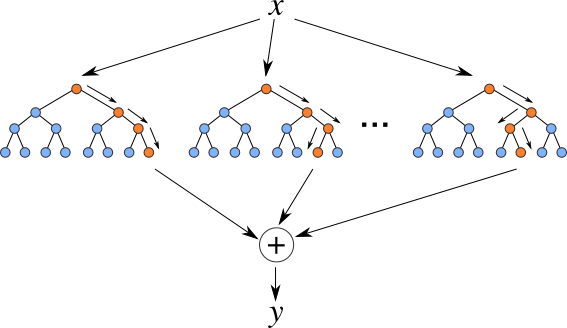
\includegraphics[width=0.8\columnwidth]{rf_ex}
					\end{center}
					\caption{Mô hình Random Forest}
				\end{figure}
		
		Random Forest là thuật toán học có giám sát nên có thể giải quyết bài toán classification.
		
		Random Forest (hay còn gọi là Rừng Ngẫu Nhiên)  được phát triển bởi Leo Breiman tại đại học California, Berkeley; là một trong những thuật toán thuộc kỹ thuật Bagging của phương pháp Ensemble Learning với mục đích dùng để phân loại bằng cách xây dựng vô số các cây quyết định (decision tree) trong thời gian huấn luyện. Đầu ra là tập hợp mô hình phân lớp của những cây riêng biệt:
		${h(X, \Theta n)}$ trong đó $\Theta n$ là những vector ngẫu nhiên phân phối độc lập như nhau và mỗi cây sẽ chọn ra được một đơn vị chọn lớp phổ biến nhất thuộc dữ liệu đầu vào X.
		
		Mỗi cây quyết định đều có những yếu tố ngẫu nhiên: Lấy ngẫu nhiên dữ liệu để xây dựng cây quyết định hoặc lấy ngẫu nhiên các thuộc tính để xây dựng cây quyết định.
		Ở bước huấn luyện Random Forest sẽ xây dựng nhiều cây quyết định, các cây quyết định có thể khác nhau. Sau đó ở bước dự đoán, với một dữ liệu mới, thì ở mỗi cây quyết định, đi từ trên xuống theo các nút điều kiện để được các dự đoán, sau đó kết quả cuối cùng được tổng hợp từ kết quả của các cây quyết định.
		
		Trong những năm gần đây, Random Forest được sử dụng khá phổ biến bởi những điểm vượt trội của nó so với các thuật toán khác: xử lý được với dữ liệu có số lượng các thuộc tính lớn, làm việc với tập dữ liệu thiếu giá trị, thường có độ chính xác cao trong phân loại, tránh được overfitting với tập dữ liệu và quá trình học nhanh.
		
		\textbf{Công cụ sử dụng:} Hàm \textit{RandomForestClassifier} trong module \textit{ensemble} của thư viện scikit-learn
		\pagebreak
	\section{Huấn luyện và tinh chỉnh mô hình}
		Sau khi đã tìm hiểu cơ sở lý thuyết của các phương pháp Học máy, chúng tôi tiến hành huấn luyện và thẩm định các bộ giá trị siêu tham số ứng với từng mô hình nhằm tìm ra bộ tham số tối ưu.
				
		Việc tinh chỉnh mô hình Học máy được thực hiện bằng cách sử dụng công cụ GridsearchCV hỗ trợ bởi thư viện scikit-learn, đánh giá qua phương pháp k-Fold Cross Validation với k=3 trên tập huấn luyện đã được tiền xử lý và vector hóa, cùng độ đo F1\_macro.
	
	
		\begin{table}[H]
			\renewcommand{\arraystretch}{1.5}
			{
				\footnotesize
				\begin{center}
					\begin{tabular}{ |m{3.4cm}|m{3.7cm}|m{3.7cm}|m{3.7cm}|}
						\hline
						\multicolumn{4}{|c|} {\rule{0pt}{20pt} \textbf{Kết quả tinh chỉnh mô hình với GridSearchCV}} \\[0.8em]
						\hline 
						\rule{0pt}{25pt}&\centering \textbf{CountVectorizer} &\centering \textbf{TfidfVectorizer}&\centering \textbf{Word2Vec} \tabularnewline
						\hline
						\multirow{2}{2em}{\textbf{LogisticRegression}} & solver = sag & solver = saga & solver = lbfgs \\
						& C = 0.1 & C = 1000 & C = 10 \\ 
						\hline 
						\multirow{2}{4em}{\textbf{MultinomialNB}} & alpha = 0.1 & alpha = 0.1 & alpha = 0.8 \\ 
						& fit\_prior = True & fit\_prior = True &fit\_prior = True\\ 
						\hline 
						\multirow{3}{1em}{\textbf{SVC}} & kernel = linear & kernel = rbf & kernel = rbf  \\
						& C = 0.1 & C = 10 & C = 10 \\ 
						& gamma = 1 & gamma = 0.1 &gamma = 0.1  \\
						\hline
						\multirow{2}{4em}{\textbf{PassiveAggressive\\Classifier}} & C = 0.001 & C = 0.1 &C = 0.01 \\
						& early\_stopping = True & early\_stopping = False & early\_stopping = False\\                         
						\hline 
						\multirow{4}{4em}{\textbf{DecisionTree\\Classifier}} & criterion = entropy & criterion = gini & criterion = entropy  \\
						& max\_depth = None & max\_depth = 32 & max\_depth = None \\ 
						& min\_sample\_leaf = 1 & min\_sample\_leaf = 2 & min\_sample\_leaf = 1  \\
						& min\_sample\_split = 2  & min\_sample\_split = 5 & min\_sample\_split = 2  \\
						\hline 
						\multirow{4}{4em}{\textbf{RandomForest\\Classifier}} & criterion = entropy & criterion = gini & criterion = entropy  \\
						& min\_sample\_split = 2 & min\_sample\_split = 5 & min\_sample\_split =  5 \\
						& min\_sample\_leaf = 1 & min\_sample\_leaf = 1 & min\_sample\_leaf =  1 \\
						& n\_estimators = 100 & n\_estimators = 400 & n\_estimators = 300 \\
						\hline
					\end{tabular}
					\caption{Bảng kết quả GridSearchCV}
				\end{center}
			}
		\end{table}

\chapter{ĐÁNH GIÁ HIỆU SUẤT MÔ HÌNH}
	\section{Các độ đo đánh giá mô hình}
	\subsection{Confusion Matrix}
		Khi đánh giá một mô hình phân lớp, để biết được cụ thể các lớp được phân loại như thế nào, lớp nào được phân loại đúng nhiều nhất, dữ liệu lớp nào thường bị phân nhầm vào lớp khác,... chúng ta thường sử dụng một ma trận được gọi là Confusion Matrix (hay còn gọi là Ma trận nhầm lẫn).
		
		\begin{figure}[H]
		\centering
		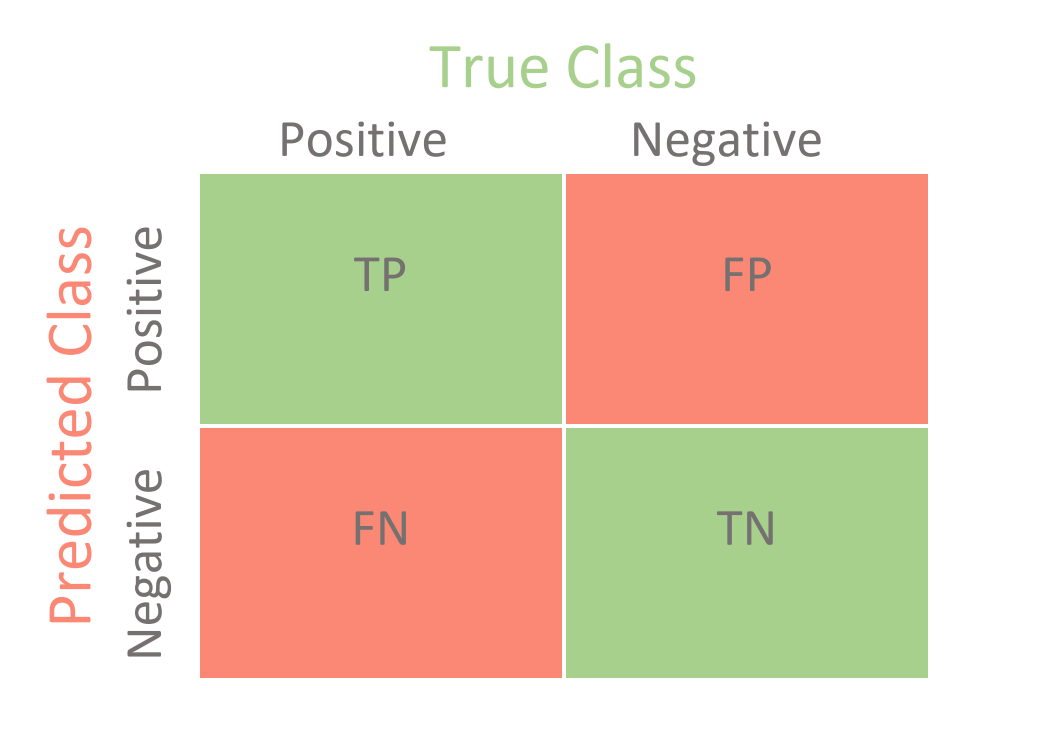
\includegraphics[width=0.47\textwidth]{confusionmatrix}
		\caption{Cấu trúc cơ bản của một Confusion Matrix}
		\end{figure}
		
		Trong bài toán phân lớp nhị phân, Confusion Matrix là một ma trận có kích thước là 2x2 (như hình 5.1), trong đó:
		\begin{itemize}
		\item \textbf{True Positive (TP):} số điểm dữ liệu có nhãn là Positive được dự đoán là Positive.
		\item \textbf{False Positive (FP):} số điểm dữ liệu có nhãn là Negative bị dự đoán là Positive.
		\item \textbf{False Negative (FN):} số điểm dữ liệu có nhãn là Positive bị dự đoán là Negative.
		\item \textbf{True Negative (TN):} số điểm dữ liệu có nhãn là Negative được dự đoán là Negative.
		\end{itemize}
		
		Một cách tổng quát, Confusion Matrix là một ma trận vuông có kích thước mỗi chiều bằng số lượng lớp dữ liệu. Giá trị tại hàng thứ i, cột thứ j là số lượng điểm lẽ ra thuộc vào class i nhưng lại được dự đoán là thuộc vào class j. Bên cạnh cách định nghĩa trên thì vẫn có một số tài liệu định nghĩa ngược lại.
		
		Để có cái nhìn rõ hơn thì Confusion Matrix còn được biểu diễn bằng cách chuẩn hóa (normalize). Việc chuẩn hóa Confusion Matrix được thực hiện bằng cách lấy từng phần tử trong mỗi hàng chia cho tổng phần tử trên hàng đó. Như vậy tổng của các phần tử trên một hàng luôn bằng 1.

		\begin{figure}[H]
			\centering
			\subfloat[Trước khi chuẩn hóa]{% 
				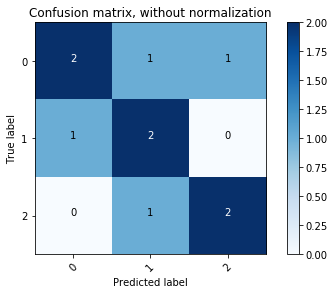
\includegraphics[width=0.48\textwidth]{ucm}} 
			\hfill
			\subfloat[Sau khi chuẩn hóa]{%
				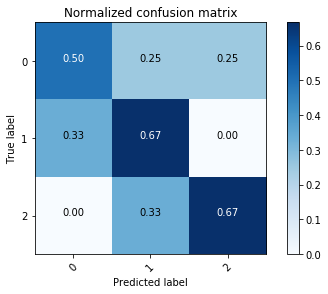
\includegraphics[width=0.48\textwidth]{ncm}} 
			\caption{Ví dụ về Confusion Matrix trước và sau khi được chuẩn hóa} 
		\end{figure}

	\subsection{Accuracy}
	Độ chính xác Accuracy là độ đo đơn giản dùng để đánh giá hiệu suất phân loại của một mô hình Học máy. Cách đánh giá này đơn giản tính tỉ lệ số lượng điểm dữ liệu được dự đoán đúng trên tổng số điểm dữ liệu trong tập kiểm thử:
	
	\centerline{$accuracy = \cfrac{TP+TN}{TP+TN+FP+FN}$}
	\vspace{1em}
	Độ đo Accuracy thường không phù hợp đối với bài toán phân loại có số lượng điểm dữ liệu giữa các lớp quá mất cân bằng, vì mô hình có xu hướng đánh giá dựa trên lớp có nhiều điểm dữ liệu hơn. Tuy nhiên đối với bộ dữ liệu sử dụng trong bài toán này thì độ đo Accuracy vẫn mang lại hiệu quả do phân bố điểm dữ liệu trên hai lớp là cân bằng.
	\subsection{Precision - Recall - F1}
	Độ đo Precision được tính bằng tỉ lệ giữa số điểm dữ liệu có nhãn là Positive được dự đoán đúng trên tổng số dự đoán Positive đưa ra bởi mô hình:
	
	\centerline{$precision = \cfrac{TP}{TP+FP}$}
	\vspace{1em}
	Độ đo Recall (còn gọi là Sensitivity hay độ phủ) được tính bằng tỉ lệ giữa số điểm dữ liệu có nhãn là Positive được dự đoán đúng trên tổng số điểm dữ liệu có nhãn là Positive:
		
	\centerline{$recall = \cfrac{TP}{TP+FN}$}
	\vspace{1em}
	
	Nếu \textbf{Precision cao} trong khi \textbf{Recall thấp}: Mô hình có độ chính xác cao trên tổng số dự đoán Positive được mô hình đưa ra, tuy nhiên nó lại có xu hướng bỏ sót nhiều điểm dữ liệu có nhãn là Positive trong thực tế.
	
	Nếu \textbf{Recall cao} trong khi \textbf{Precision thấp}: Mô hình có độ phủ tốt trên các nhãn Positive, tuy nhiên độ chính xác của kết quả dự đoán các điểm dữ liệu này lại không cao.
	
	Để thể hiện sự tổng hòa giữa Precision và Recall, một độ đo khác được sử dụng để đánh giá mô hình phân lớp, đó là độ đo F1 và được tính bằng trung bình điều hòa của Precision và Recall:  
	
	\centerline{$F_1 = 2 \times \cfrac{precision\cdot recall}{precision+recall}$}
	\vspace{1em}
	Độ đo $F_1$ thường được dùng khi chúng ta cần sự đồng đều giữa precision và recall hoặc khi bộ dữ liệu quá mất cân bằng. Vì vậy nó được sử dụng rất phổ biến trong các bài toán thực tế và trong nghiên cứu khoa học.
	
	\subsection{Đường cong ROC và chỉ số AUC}
	Đường cong ROC (Receiver Operating Characteristic Curve) là một đồ thị đánh giá hiệu suất thường được sử dụng trong bài toán phân lớp nhị phân. Ứng dụng đầu tiên của nó là cho việc nghiên cứu các hệ thống nhận diện trong việc phát hiện các tín hiệu radio khi có sự hiện diện của nhiễu vào thập niên 1940, sau sự kiện cuộc tấn công Trân Châu Cảng. 
	
	Đường cong ROC thường được biểu diễn bằng cặp chỉ số (TPR, FPR) tại mỗi ngưỡng với TPR là trục tung và FPR là trục hoành. Trong đó:
	\begin{itemize}
	\item $TPR = Recall = \cfrac{TP}{TP+FN}$
	\item $FPR = \cfrac{FP}{TN+FP}\vspace{1em}$: tỉ lệ giữa số điểm dữ liệu có nhãn Negative bị dự đoán sai trên tổng số điểm dữ liệu có nhãn là Negative.
	\end{itemize}
	
	Đây chính là các chỉ số dùng để tính toán hiệu suất phân loại của mô hình. Để hợp chúng lại thành 1 chỉ số duy nhất, ta sử dụng đường cong ROC để hiển thị từng cặp (TPR, FPR) cho các ngưỡng khác nhau với mỗi điểm trên đường cong biểu diễn 1 cặp (TPR, FPR) cho 1 ngưỡng, sau đó tính chỉ số AUC cho đường cong này. 
	
	Chỉ số AUC (Area under the curve) chính là diện tích không gian bên dưới đường cong ROC, là con số thể hiện hiệu suất phân loại của mô hình. 
	
	AUC càng gần về 1 (ROC hội tụ về góc trên bên trái) thì mô hình càng phân loại chính xác, AUC càng gần về 0.5 (ROC hội tụ về đường chéo) thì hiệu suất phân loại càng tệ. Nếu AUC càng gần về 0 thì mô hình sẽ phân loại ngược kết quả (phân loại Positive thành Negative và ngược lại)
	
			\begin{figure}[H]
				\centering
				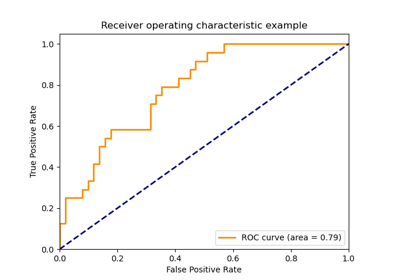
\includegraphics[width=1\textwidth]{roc_auc}
				\caption{Ví dụ về đường cong ROC và AUC}
			\end{figure}
	
	\pagebreak
	\section{Kết quả đánh giá hiệu suất mô hình}
		Khi đã tìm được những giá trị siêu tham số tốt nhất của từng mô hình trên từng bộ vector hóa, chúng tôi tiến hành dự đoán các điểm dữ liệu trong tập kiểm thử và thu được kết quả đánh giá dưới đây.
	
	\begin{table}[H]
			\renewcommand{\arraystretch}{1.5}
			\small
			\begin{center}
				\begin{tabular}{ | P{13.2em} | P{3.2cm}| P{3cm} | P{2.5cm} |} 
				\hline
			      & \textbf{CountVectorizer} & \textbf{TfidfVectorizer} & \textbf{Word2Vec} \\ 
				\hline
				\textbf{LogisticRegression} & \textbf{0.9242} & 0.9533 & 0.9154\\ 
				\hline
				\textbf{MultinomialNB} & 0.9091 & 0.9129 & 0.7936 \\
				\hline
				\textbf{SVC} & 0.9053 & 0.9520 & \textbf{0.9249} \\
				\hline
				\textbf{PassiveAggressiveClassifier} & 0.9154 & \textbf{0.9552} & 0.8958 \\
				\hline
				\textbf{DecisionTreeClassifier} & 0.8182 & 0.7891 & 0.7841 \\
				\hline
				\textbf{RandomForestClassifer} & 0.9066 & 0.9104 & 0.8996 \\
				\hline
				\end{tabular}
			\end{center}
			\caption{Bảng tổng hợp kết quả đánh giá độ chính xác (Accuracy) của các mô hình}
		\end{table}
		\hfill
		\begin{figure}[H]
			\centering
			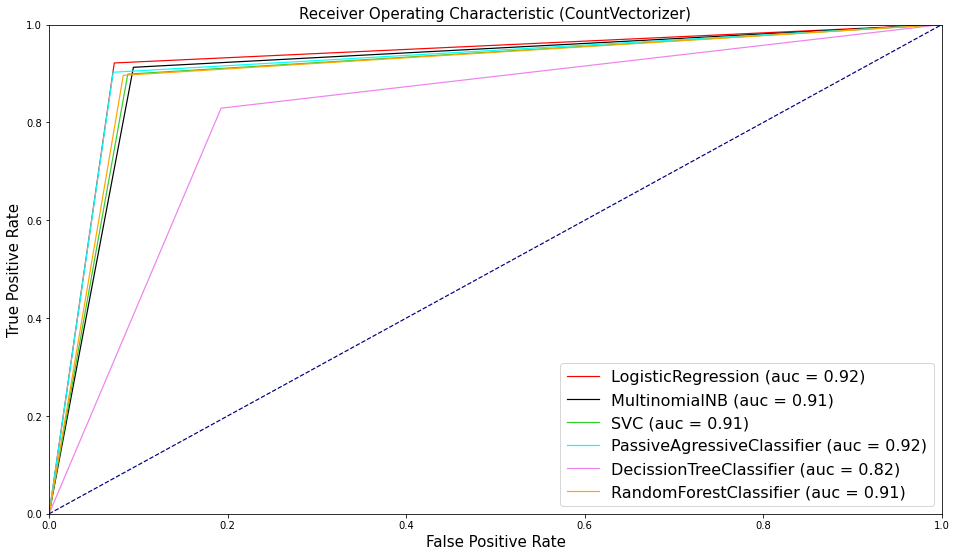
\includegraphics[width=1\textwidth]{cvroc}
			\caption{Đường cong ROC cho bộ CountVectorizer}
		\end{figure}
		
		\begin{figure}[H]
			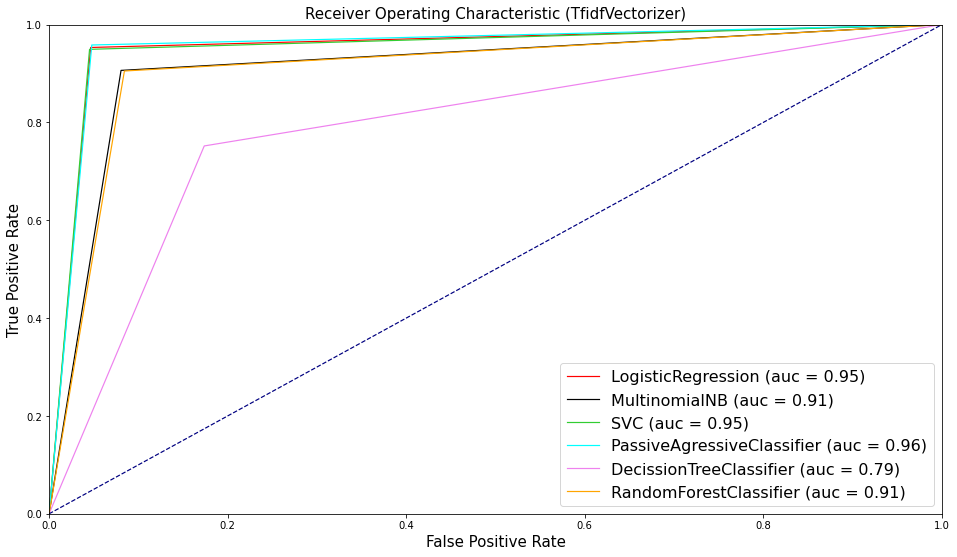
\includegraphics[width=1\textwidth]{tfroc}
			\caption{Đường cong ROC cho bộ TfidfVectorizer} 
		\end{figure}
		\hfill
		\begin{figure}[H]
			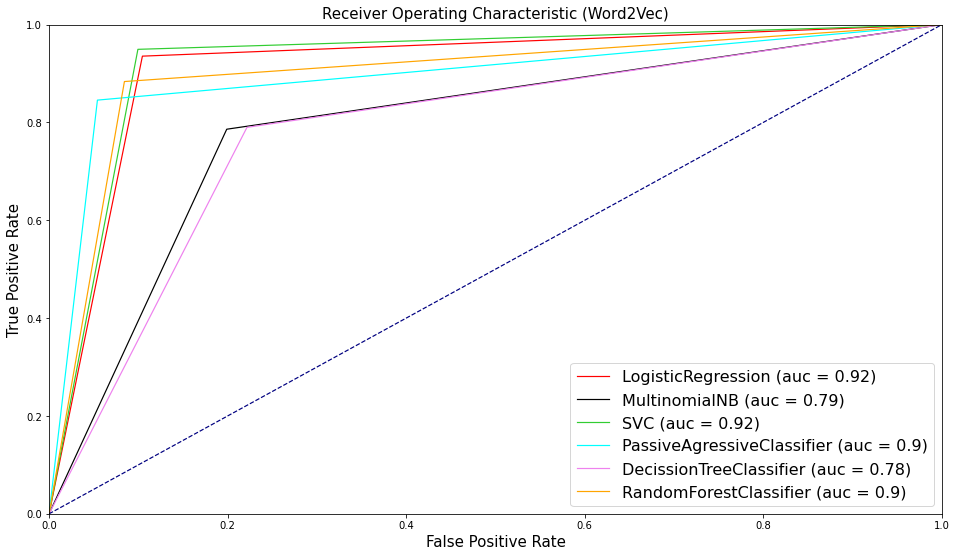
\includegraphics[width=1\textwidth]{w2vroc}
			\caption{Đường cong ROC cho bộ Word2Vec} 
		\end{figure}
		\pagebreak
	
	\subsection{Kết quả đánh giá LogisticRegression}
		\begin{figure}[H]
			\subfloat[\textbf{CountVectorizer}]{% 
				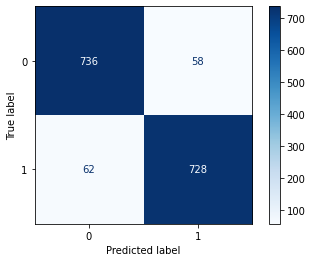
\includegraphics[width=0.33\textwidth]{cvlr}} 
			\hfill
			\subfloat[\textbf{TfidfVectorizer}]{%
				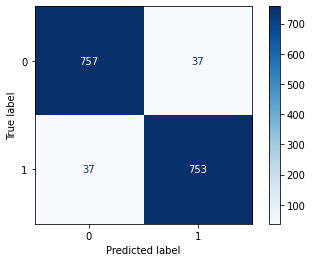
\includegraphics[width=0.33\textwidth]{tflr}} 
			\hfill
			\subfloat[\textbf{Word2Vec}]{%
				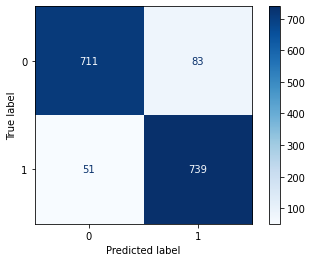
\includegraphics[width=0.33\textwidth]{w2vlr}}
			\caption{Confusion Matrix LogisticRegression} 
		\end{figure}

		\begin{table}[H]
			\renewcommand{\arraystretch}{1.5}
		
			\begin{center}
			\subfloat[\textbf{CountVectorizer}]{% 
				\begin{tabular}{ | P{5em} | P{2cm}| P{3cm} | P{3cm} | P{3cm} |} 
				\hline
      			  & precision & recall & f1-score & support \\ 
				\hline
				0 & 0.92 & 0.93 & 0.92 & 794\\ 
				\hline
				1 & 0.93 & 0.92 & 0.92 & 790\\
				\hline
				macro avg & 0.92 & 0.92 & 0.92 & 1584\\
				\hline
				\end{tabular}} 
			\hfill
			\hrule
			\vspace{3ex}
			\subfloat[\textbf{TfidfVectorizer}]{%
				\begin{tabular}{ | P{5em} | P{2cm}| P{3cm} | P{3cm} | P{3cm} |} 
				\hline
      			  & precision & recall & f1-score & support \\ 
				\hline
				0 & 0.95 & 0.95 & 0.95 & 794\\ 
				\hline
				1 & 0.95 & 0.95 & 0.95 & 790\\
				\hline
				macro avg & 0.95 & 0.95 & 0.95 & 1584\\
				\hline
				\end{tabular}} 
			\hfill
			\hrule
			\vspace{3ex}
			\subfloat[\textbf{Word2Vec}]{% 
				\begin{tabular}{ | P{5em} | P{2cm}| P{3cm} | P{3cm} | P{3cm} |} 
				\hline
      			  & precision & recall & f1-score & support \\ 
				\hline
				0 & 0.93 & 0.90 & 0.91 & 794\\
				\hline
				1 & 0.90 & 0.94 & 0.92 & 790\\ 
				\hline

				macro avg & 0.92 & 0.92 & 0.92 & 1584\\
				\hline
				
				\end{tabular}}
			\hrule
			\end{center}
			
			\caption{Classification report LogisticRegression}
		\end{table}



\subsection{Kết quả đánh giá MultinomialNB}

\begin{figure}[H]
	\subfloat[\textbf{CountVectorizer}]{% 
		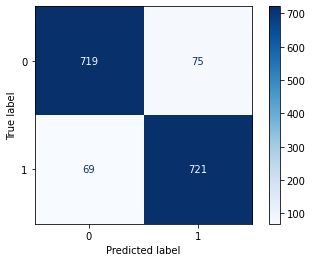
\includegraphics[width=0.33\textwidth]{cvnb}} 
	\hfill
	\subfloat[\textbf{TfidfVectorizer}]{%
		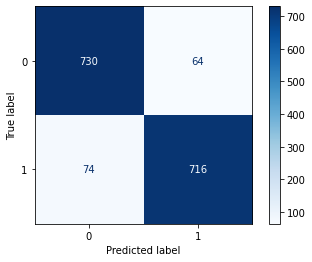
\includegraphics[width=0.33\textwidth]{tfnb}} 
	\hfill
	\subfloat[\textbf{Word2Vec}]{%
		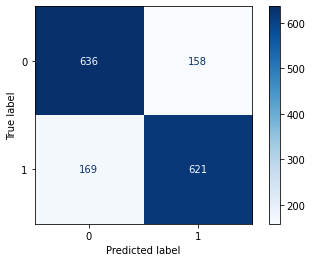
\includegraphics[width=0.33\textwidth]{w2vnb}}
	\caption{Confusion Matrix MultinomialNB} 
\end{figure}

\begin{table}[H]
	\renewcommand{\arraystretch}{1.5}
	\begin{center}
	\subfloat[\textbf{CountVectorizer}]{% 
		\begin{tabular}{ | P{5em} | P{2cm}| P{3cm} | P{3cm} | P{3cm} |} 
		\hline
	      & precision & recall & f1-score & support \\ 
		\hline
		0 & 0.91 & 0.91 & 0.91 & 794\\
		\hline
		1 & 0.91 & 0.91 & 0.91 & 790\\ 
		\hline

		macro avg & 0.91 & 0.91 & 0.91 & 1584\\
		\hline
		\end{tabular}} 
	\hfill
	\hrule
	\vspace{3ex}
	\subfloat[\textbf{TfidfVectorizer}]{% 
		\begin{tabular}{ | P{5em} | P{2cm}| P{3cm} | P{3cm} | P{3cm} |} 
		\hline
	      & precision & recall & f1-score & support \\ 
		\hline
		0 & 0.91 & 0.92 & 0.91 & 794\\
		\hline
		1 & 0.92 & 0.91 & 0.91 & 790\\ 
		\hline

		macro avg & 0.91 & 0.91 & 0.91 & 1584\\
		\hline
		\end{tabular}} 
	\hfill
	\hrule
	\vspace{3ex}
	\subfloat[\textbf{Word2Vec}]{% 
		\begin{tabular}{ | P{5em} | P{2cm}| P{3cm} | P{3cm} | P{3cm} |} 
		\hline
	      & precision & recall & f1-score & support \\ 
		\hline
		0 & 0.79 & 0.80 & 0.80 & 794\\
		\hline
		1 & 0.80 & 0.79 & 0.79 & 790\\ 
		\hline

		macro avg & 0.79 & 0.79 & 0.79 & 1584\\
		\hline
		
		\end{tabular}}
	\hrule
	\end{center}
	
	\caption{Classification report MultinomialNB}
\end{table}

\subsection{Kết quả đánh giá SVC}

\begin{figure}[H]
	\subfloat[\textbf{CountVectorizer}]{% 
		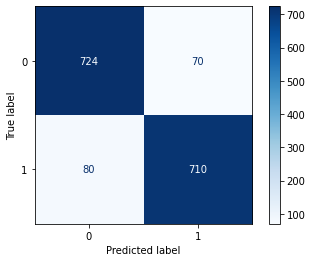
\includegraphics[width=0.33\textwidth]{cvsvc}} 
	\hfill
	\subfloat[\textbf{TfidfVectorizer}]{%
		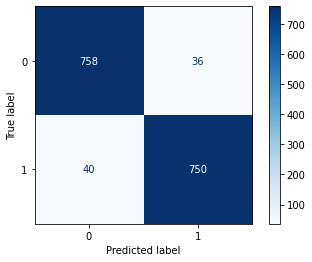
\includegraphics[width=0.33\textwidth]{tfsvc}} 
	\hfill
	\subfloat[\textbf{Word2Vec}]{%
		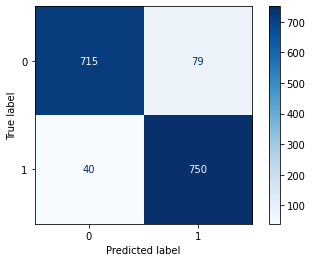
\includegraphics[width=0.33\textwidth]{w2vsvc}}
	\caption{Confusion Matrix SVC} 
\end{figure}

\begin{table}[H]
	\renewcommand{\arraystretch}{1.5}
	\begin{center}
	\subfloat[\textbf{CountVectorizer}]{% 
		\begin{tabular}{ | P{5em} | P{2cm}| P{3cm} | P{3cm} | P{3cm} |} 
		\hline
	      & precision & recall & f1-score & support \\ 
		\hline
		0 & 0.90 & 0.91 & 0.91 & 794\\
		\hline
		1 & 0.91 & 0.90 & 0.90 & 790\\ 
		\hline

		macro avg & 0.91 & 0.91 & 0.91 & 1584\\
		\hline
		\end{tabular}} 
	\hfill
	\hrule
	\vspace{3ex}
	\subfloat[\textbf{TfidfVectorizer}]{% 
		\begin{tabular}{ | P{5em} | P{2cm}| P{3cm} | P{3cm} | P{3cm} |} 
		\hline
	      & precision & recall & f1-score & support \\ 
		\hline
		0 & 0.95 & 0.95 & 0.95 & 794\\ 
		\hline
		1 & 0.95 & 0.95 & 0.95 & 790\\
		\hline
		macro avg & 0.95 & 0.95 & 0.95 & 1584\\
		\hline
		\end{tabular}} 
	\hfill
	\hrule
	\vspace{3ex}
	\subfloat[\textbf{Word2Vec}]{% 
		\begin{tabular}{ | P{5em} | P{2cm}| P{3cm} | P{3cm} | P{3cm} |} 
		\hline
	      & precision & recall & f1-score & support \\ 
		\hline
		0 & 0.95 & 0.90 & 0.92 & 794\\
		\hline
		1 & 0.90 & 0.95 & 0.93 & 790\\ 
		\hline

		macro avg & 0.93 & 0.92 & 0.92 & 1584\\
		\hline
		
		\end{tabular}}
	\hrule
	\end{center}
	
	\caption{Classification report SVC}
\end{table}

\subsection{Kết quả đánh giá PassiveAggressiveClassifier}

\begin{figure}[H]
	\subfloat[\textbf{CountVectorizer}]{% 
		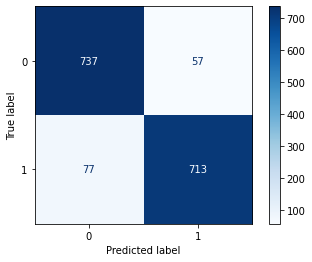
\includegraphics[width=0.33\textwidth]{cvpa}} 
	\hfill
	\subfloat[\textbf{TfidfVectorizer}]{%
		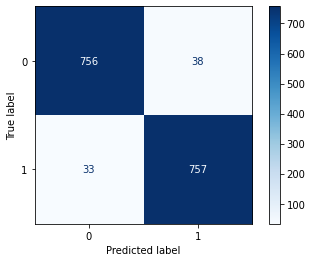
\includegraphics[width=0.33\textwidth]{tfpa}} 
	\hfill
	\subfloat[\textbf{Word2Vec}]{%
		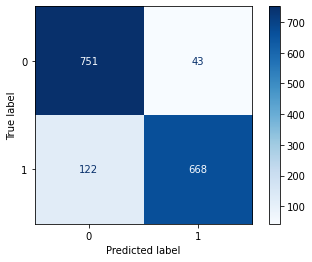
\includegraphics[width=0.33\textwidth]{w2vpa}}
	\caption{Confusion Matrix PassiveAggressiveClassifier} 
\end{figure}

\begin{table}[H]
	\renewcommand{\arraystretch}{1.5}
	\begin{center}
	\subfloat[\textbf{CountVectorizer}]{% 
		\begin{tabular}{ | P{5em} | P{2cm}| P{3cm} | P{3cm} | P{3cm} |} 
		\hline
	      & precision & recall & f1-score & support \\ 
		\hline
		0 & 0.91 & 0.93 & 0.92 & 794\\
		\hline
		1 & 0.93 & 0.90 & 0.91 & 790\\ 
		\hline

		macro avg & 0.92 & 0.92 & 0.92 & 1584\\
		\hline
		\end{tabular}} 
	\hfill
	\hrule
	\vspace{3ex}
	\subfloat[\textbf{TfidfVectorizer}]{% 
		\begin{tabular}{ | P{5em} | P{2cm}| P{3cm} | P{3cm} | P{3cm} |} 
		\hline
	      & precision & recall & f1-score & support \\ 
		\hline
		0 & 0.96 & 0.95 & 0.96 & 794\\
		\hline
		1 & 0.95 & 0.96 & 0.96 & 790\\ 
		\hline

		macro avg & 0.96 & 0.96 & 0.96 & 1584\\
		\hline
		\end{tabular}} 
	\hfill
	\hrule
	\vspace{3ex}
	\subfloat[\textbf{Word2Vec}]{% 
		\begin{tabular}{ | P{5em} | P{2cm}| P{3cm} | P{3cm} | P{3cm} |} 
		\hline
	      & precision & recall & f1-score & support \\ 
		\hline
		0 & 0.86 & 0.95 & 0.90 & 794\\
		\hline
		1 & 0.94 & 0.85 & 0.89 & 790\\ 
		\hline
	
		macro avg & 0.90 & 0.90 & 0.90 & 1584\\
		\hline
		
		\end{tabular}}
	\hrule
	\end{center}
	
	\caption{Classification report PassiveAggressiveClassifier}
\end{table}

\subsection{Kết quả đánh giá DecisionTreeClassifier}

\begin{figure}[H]
	\subfloat[\textbf{CountVectorizer}]{% 
		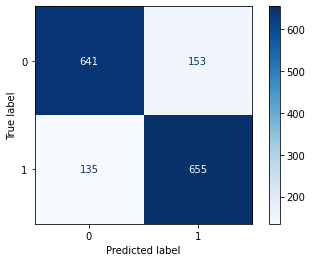
\includegraphics[width=0.33\textwidth]{cvdtree}} 
	\hfill
	\subfloat[\textbf{TfidfVectorizer}]{%
		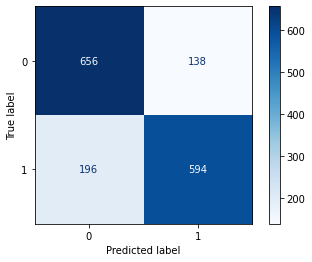
\includegraphics[width=0.33\textwidth]{tfdtree}} 
	\hfill
	\subfloat[\textbf{Word2Vec}]{%
		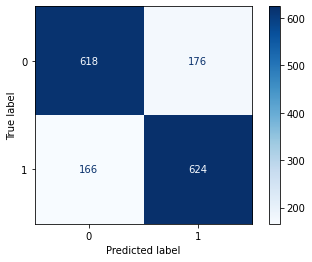
\includegraphics[width=0.33\textwidth]{w2vdtree}}
	\caption{Confusion Matrix DecisionTreeClassifier} 
\end{figure}

\begin{table}[H]
	\renewcommand{\arraystretch}{1.5}
	\begin{center}
	\subfloat[\textbf{CountVectorizer}]{% 
		\begin{tabular}{ | P{5em} | P{2cm}| P{3cm} | P{3cm} | P{3cm} |} 
		\hline
	      & precision & recall & f1-score & support \\ 
		\hline
		0 & 0.83 & 0.81 & 0.82 & 794\\ 
		\hline
		1 & 0.81 & 0.83 & 0.82 & 790\\
		\hline
		macro avg & 0.82 & 0.82 & 0.82 & 1584\\
		\hline
		\end{tabular}} 
	\hfill
	\hrule
	\vspace{3ex}
	\subfloat[\textbf{TfidfVectorizer}]{% 
		\begin{tabular}{ | P{5em} | P{2cm}| P{3cm} | P{3cm} | P{3cm} |} 
		\hline
	      & precision & recall & f1-score & support \\ 
		\hline
		0 & 0.77 & 0.83 & 0.80 & 794\\
		\hline
		1 & 0.81 & 0.75 & 0.78 & 790\\ 
		\hline

		macro avg & 0.79 & 0.79 & 0.79 & 1584\\
		\hline
		\end{tabular}} 
	\hfill
	\hrule
	\vspace{3ex}
	\subfloat[\textbf{Word2Vec}]{% 
		\begin{tabular}{ | P{5em} | P{2cm}| P{3cm} | P{3cm} | P{3cm} |} 
		\hline
	      & precision & recall & f1-score & support \\ 
		\hline
		0 & 0.79 & 0.78 & 0.78 & 794\\
		\hline
		1 & 0.78 & 0.79 & 0.78 & 790\\ 
		\hline

		macro avg & 0.78 & 0.78 & 0.78 & 1584\\
		\hline
		\end{tabular}}
	\hrule
	\end{center}
	
	\caption{Classification report DecisionTreeClassifier}
\end{table}

\subsection{Kết quả đánh giá RandomForestClassifier}

\begin{figure}[H]
	\subfloat[\textbf{CountVectorizer}]{% 
		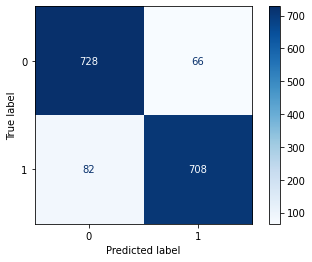
\includegraphics[width=0.33\textwidth]{cvrf}} 
	\hfill
	\subfloat[\textbf{TfidfVectorizer}]{%
		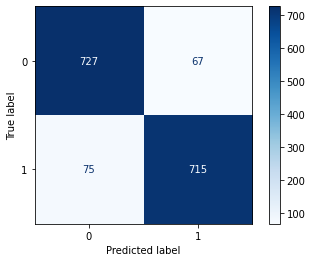
\includegraphics[width=0.33\textwidth]{tfrf}} 
	\hfill
	\subfloat[\textbf{Word2Vec}]{%
		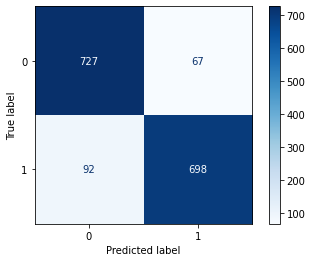
\includegraphics[width=0.33\textwidth]{w2vrf}}
	\caption{Confusion Matrix RandomForestClassifier} 
\end{figure}

\begin{table}[H]
	\renewcommand{\arraystretch}{1.5}
	\begin{center}
	\subfloat[\textbf{CountVectorizer}]{% 
		\begin{tabular}{ | P{5em} | P{2cm}| P{3cm} | P{3cm} | P{3cm} |} 
		\hline
	      & precision & recall & f1-score & support \\ 
		\hline
		0 & 0.90 & 0.92 & 0.91 & 794\\
		\hline
		1 & 0.91 & 0.90 & 0.91 & 790\\ 
		\hline

		macro avg & 0.91 & 0.91 & 0.91 & 1584\\
		\hline
		\end{tabular}} 
	\hfill
	\hrule
	\vspace{3ex}
	\subfloat[\textbf{TfidfVectorizer}]{% 
		\begin{tabular}{ | P{5em} | P{2cm}| P{3cm} | P{3cm} | P{3cm} |} 
		\hline
	      & precision & recall & f1-score & support \\ 
		\hline
		0 & 0.91 & 0.92 & 0.91 & 794\\ 
		\hline
		1 & 0.91 & 0.91 & 0.91 & 790\\
		\hline
		macro avg & 0.91 & 0.91 & 0.91 & 1584\\
		\hline
		\end{tabular}} 
	\hfill
	\hrule
	\vspace{3ex}
	\subfloat[\textbf{Word2Vec}]{% 
		\begin{tabular}{ | P{5em} | P{2cm}| P{3cm} | P{3cm} | P{3cm} |} 
		\hline
	      & precision & recall & f1-score & support \\
		\hline
		0 & 0.89 & 0.92 & 0.90 & 794\\
		\hline
		1 & 0.91 & 0.88 & 0.90 & 790\\ 
		\hline

		macro avg & 0.90 & 0.90 & 0.90 & 1584\\
		\hline
		
		\end{tabular}}
	\hrule
	\end{center}
	
	\caption{Classification report RandomForestClassifier}
\end{table}

\chapter{PHÂN TÍCH LỖI VÀ HƯỚNG PHÁT TRIỂN}
\section{Phân tích lỗi mô hình tốt nhất}

Qua kết quả đánh giá tổng hợp thu được, mô hình PassiveAggressiveClassifier cho hiệu suất cao nhất trên bộ TfidfVectorizer.
\begin{figure}[H]
	\centering
	\captionsetup{width=0.7\textwidth}
	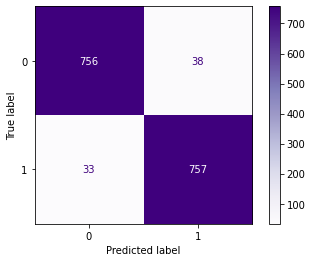
\includegraphics[width=0.6\textwidth]{tfpa_2}
	\caption{Confusion Matrix của mô hình Passive Aggressive Classifier với TfidfVectorizer}
\end{figure}
Nhìn sơ lược qua Confusion Matrix, dữ liệu hầu hết hội tụ về đường chéo của ma trận, chứng tỏ hiệu suất phân loại của mô hình là rất tốt. Tuy nhiên vẫn có một số điểm dữ liệu mô hình dự đoán không chính xác, cụ thể:
\begin{itemize}
\item Có 38 điểm dữ liệu có nhãn là FAKE (0) bị mô hình dự đoán là REAL (1)
\item Có 33 điểm dữ liệu có nhãn là REAL (1) bị mô hình dự đoán là FAKE (0)
\end{itemize}

Tỉ lệ lỗi của mô hình: $(33+38)/1584 ≈ 0.0448 = 4.48\%$. Trong đó mô hình bị lỗi False Negative nhiều hơn lỗi False Positive.

Để tìm hiểu nguyên nhân gây ra lỗi, chúng tôi xem qua những từ xuất hiện nhiều ở cả 2 nhãn trên toàn bộ tập dữ liệu và ở các điểm dữ liệu bị lỗi False Positive và False Negative để đưa ra so sánh.
\begin{figure}[H]
	\centering
	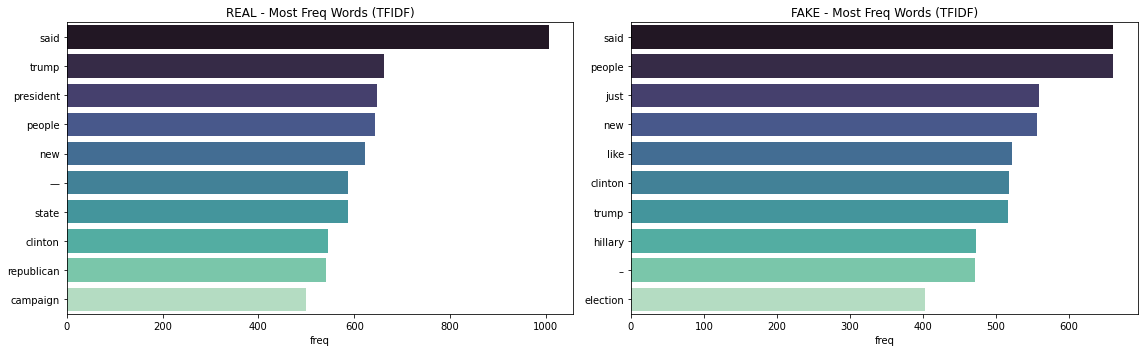
\includegraphics[width=1\textwidth]{frequentdata}
	\caption{Những từ xuất hiện nhiều ở hai nhãn của tập dữ liệu}
\end{figure}

\begin{figure}[H]
	\subfloat[\textbf{Lỗi False Negative}]{% 
		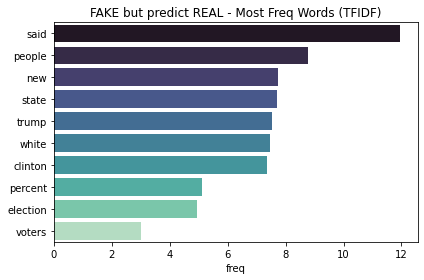
\includegraphics[width=0.5\textwidth]{fn1gram}} 
	\hfill
	\subfloat[\textbf{Lỗi False Positive}]{%
		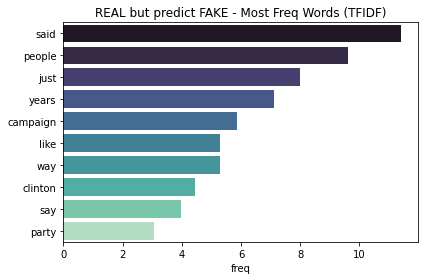
\includegraphics[width=0.5\textwidth]{fp1gram}} 
	\caption{Những từ xuất hiện nhiều ở lỗi False Negative và False Positive trên tập kiểm thử} 
\end{figure}

\textbf{Nhận xét:} Những từ `said', `people', `new', `trump' đều có tần suất xuất hiện rất cao ở cả hai nhãn của bộ dữ liệu. Qua hình 6.3, có thể thấy những từ này ảnh hưởng lớn đến mô hình, khiến mô hình bị nhầm lẫn giữa hai nhãn và đưa ra dự đoán sai.

\textbf{Hướng giải quyết:} Có thể hạn chế những tác động của những từ gây nhiễu bằng cách loại bỏ chúng hoàn toàn hoặc giảm chiều dữ liệu. Tuy nhiên, lúc này cần những phương pháp mạnh hơn để hoạt động hiệu quả trên bộ dữ liệu đã thu gọn.

\section{Hướng phát triển}
Trong tương lai có thể áp dụng các phương pháp Ensemble Learning như XGBoost, Adaboost,.. và mô hình Neural Network như LSTM, RNN,... để có thể cải thiện độ chính xác trên bộ dữ liệu.

Ngoài ra, việc sử dụng các pretrained model khác như Glove, StanfordNLP, BERT với các mô hình trên cũng cần được nghiên cứu và có khả năng ứng dụng vào thực tế.

\chapter*{KẾT LUẬN}
\addcontentsline{toc}{chapter}{KẾT LUẬN}

Báo cáo đồ án của chúng tôi đã trình bày một cách ngắn gọn về cơ sở lý thuyết của các phương pháp Học máy và các kỹ thuật tiền xử lý và vector hóa dữ liệu được sử dụng. Qua đó, chúng tôi xây dựng và tinh chỉnh các mô hình Học máy dựa trên các bộ vector hóa dữ liệu khác nhau.

Do hạn chế về tài nguyên và thời gian, chúng tôi chỉ có thể thử nghiệm một số lượng nhất định giá trị tham số của các mô hình, vì vậy các mô hình sau khi tinh chỉnh có thể chưa là tốt nhất. Sau cùng, chúng tôi mong muốn có thể đưa ra bộ tham số tốt nhất của từng mô hình trên từng bộ vector hóa cụ thể, nhằm thực hiện việc so sánh và đánh giá một cách khách quan nhất về hiệu suất phân loại giữa các mô hình trên bộ dữ liệu.

Thông qua kết quả đánh giá hiệu suất mô hình, chúng tôi nhận thấy khả năng nhận diện và phân loại tin giả trên bộ dữ liệu của các phương pháp Học máy đều khá tốt với hiệu suất trung bình là 89,25\%. Trong đó, phương pháp Decision Tree cho kết quả thấp nhất trên bộ Word2Vec với độ chính xác 78,41\%. Phương pháp Passive Aggressive cho hiệu suất cao nhất trên bộ TfidfVectorizer với độ chính xác 95,52\%, do đó có thể được xem xét để ứng dụng vào trong thực tiễn.

Các bộ vector hóa dữ liệu cũng ảnh hưởng đến hiệu suất của các mô hình. Trong đó, hiệu suất trung bình của các mô hình với CountVectorizer là 89,65\% , với TfidfVectorizer là 91,22\% và với Word2Vec là 86,89\%. Bộ TfidfVectorizer mang lại hiệu suất cao hơn hai mô hình còn lại, có thể xem xét làm dữ liệu đầu vào khi thử nghiệm những phương pháp mạnh hơn.

Để tối ưu hiệu suất phân loại, trong tương lai chúng tôi dự định áp dụng kỹ thuật giảm chiều dữ liệu kết hợp với các kỹ thuật Boosting tiêu biểu trong Ensemble Learning như XGBoost, Adaboost và Gradient Boosting. Cùng với đó, chúng tôi cũng xem xét áp dụng những phương pháp Học Sâu gồm các mạng neural LSTM, RNN,... nhất là khi lượng dữ liệu tăng lên đáng kể.

Một số pretrain-model State-of-the-art như Glove, Transformer, StanfordNLP hay BERT có thể được xem xét áp dụng để trích xuất các đặc trưng một cách tốt hơn. Những mô hình như Transformer hay BERT có thể được ưu tiên hàng đầu vì chúng đã được huấn luyện rất nhiều để nhận diện ngữ cảnh trước khi đưa ra bộ vector embedding cho một từ nào đó. Các mô hình này còn giúp tiết kiệm thời gian, năng lực tính toán và dễ dàng thực hiện những tinh chỉnh hậu xử lý sau cùng.


\newpage
\renewcommand{\bibname}{\bf \LARGE \quad DANH MỤC TÀI LIỆU THAM KHẢO}
\addcontentsline{toc}{chapter}{DANH MỤC TÀI LIỆU THAM KHẢO}
\baselineskip
18pt
\begin{thebibliography}{99}
	%1
	\bibitem{} Sairamvinay Vijayaraghavan, Ye Wang, Zhiyuan Guo, John Voong, Wenda Xu, Armand Nasseri, Jiaru Cai, Linda Li, Kevin Vuong, Eshan Wadhwa,
	\textit{Fake News Detection with Different Models}.
	
	\url{https://arxiv.org/abs/2003.04978}
	
	%2
	\bibitem{}Taylor Onate Egerton, Ezekiel Promise Sochima, \textit{Application of Supervised Machine Learning Algorithms to Detect Online Fake News}.
	
	\url{https://www.researchgate.net/publication/339299161_Application_of_Supervised_Machine_Learning_Algorithms_to_Detect_Online_Fake_News}
	
	%3
	\bibitem{}Iftikhar Ahmad, Muhammad Yousaf, Suhail Yousaf, and Muhammad Ovais Ahmad
	\textit{Fake News Detection Using Machine Learning Ensemble Methods}
	
	\url{https://www.hindawi.com/journals/complexity/2020/8885861/}
	
	%4
	\bibitem{} Koby Crammer, Ofer Dekel,Joseph Keshet, Shai Shalev-Shwartz, Yoram Singer (2006),
	\textit{Online Passive-Aggressive Algorithms}.

	\url{https://jmlr.csail.mit.edu/papers/volume7/crammer06a/crammer06a.pdf}

	%5
	\bibitem{}Obinna Chilezie Njoku,
	\textit{Decision Trees and Their Application for Classification and Regression Problems}
	
	\url{https://bearworks.missouristate.edu/theses/3406/}
	
	%6
	\bibitem{}Niklas Donges, 
	\textit{The Random Forest Algorithm: A Complete Guide}
	
	\url{https://builtin.com/data-science/random-forest-algorithm}
	
	%7
	\bibitem{}Hussain Mujtaba, 
	\textit{An Introduction to Bag of Words (BoW) | What is Bag of Words?}
	
	\url{https://www.mygreatlearning.com/blog/bag-of-words}
	
	%8
	\bibitem{} Radim {\v R}eh{\r u}{\v r}ek and Petr Sojka, \textit{Software Framework for Topic Modelling with Large Corpora}.
	
	\url{https://radimrehurek.com/gensim/models/word2vec.html}
	
	%9
	\bibitem{} Vũ Hữu Tiệp, \textit{Machine Learning cơ bản}.
	
	\url{https://machinelearningcoban.com/}
	
	%10
	\bibitem{}Pedregosa, F. and Varoquaux, G. and Gramfort, A. and Michel, V.
	         and Thirion, B. and Grisel, O. and Blondel, M. and Prettenhofer, P.
	         and Weiss, R. and Dubourg, V. and Vanderplas, J. and Passos, A. and
	         Cournapeau, D. and Brucher, M. and Perrot, M. and Duchesnay, E., \textit{Scikit-learn: Machine Learning in {P}ython}.
	         
	\url{https://scikit-learn.org/stable/}
	

	
\end{thebibliography}

\end{document} 